\documentclass[useAMS,usenatbib,referee]{biom}
%\documentclass[useAMS,usenatbib,referee]{biom}
%
%
%  Papers submitted to Biometrics should ALWAYS be prepared
%  using the referee option!!!!
%
%
% If your system does not have the AMS fonts version 2.0 installed, then
% remove the useAMS option.
%
% useAMS allows you to obtain upright Greek characters.
% e.g. \umu, \upi etc.  See the section on "Upright Greek characters" in
% this guide for further information.
%
% If you are using AMS 2.0 fonts, bold math letters/symbols are available
% at a larger range of sizes for NFSS release 1 and 2 (using \boldmath or
% preferably \bmath).
%
% The usenatbib command allows the use of Patrick Daly's natbib package for
% cross-referencing.
%
% If you wish to typeset the paper in Times font (if you do not have the
% PostScript Type 1 Computer Modern fonts you will need to do this to get
% smoother fonts in a PDF file) then uncomment the next line
% \usepackage{Times}
%%%%% AUTHORS - PLACE YOUR OWN MACROS HERE %%%%%

\usepackage[figuresright]{rotating}
\usepackage{tikz}
\usepackage{amsmath, amssymb}
\usepackage[hyphens]{url} % not crucial - just used below for the URL
\usepackage{hyperref}
\usepackage[utf8]{inputenc}
\usepackage{graphicx}
\usepackage{longtable}
\usepackage{booktabs}
\def\Fsc{{\cal F}}
\def\Isc{{\cal I}}
%% \raggedbottom % To avoid glue in typesetteing, sbs>>

% tightlist command for lists without linebreak
\providecommand{\tightlist}{%
  \setlength{\itemsep}{0pt}\setlength{\parskip}{0pt}}
%%%%%%%%%%%%%%%%%%%%%%%%%%%%%%%%%%%%%%%%%%%%%%%%

\setcounter{footnote}{2}

\title[]{Evaluation of longitudinal surrogate markers}

\author{ Denis Agniel \email{\href{mailto:dagniel@rand.org}{\nolinkurl{dagniel@rand.org}}} \\ RAND Corporation  \and
		 Layla Parast \email{\href{mailto:parast@rand.org}{\nolinkurl{parast@rand.org}}} \\ RAND Corporation 
	   }

\begin{document}

\date{{\it Received Mar} 2019}

\pagerange{\pageref{firstpage}--\pageref{lastpage}} \pubyear{2019}

\volume{0}
\artmonth{January}
\doi{0000-0000-0000}

%  This label and the label ``lastpage'' are used by the \pagerange
%  command above to give the page range for the article

\label{firstpage}

%  pub the summary here

\begin{abstract}
The text of your summary. Should not exceed 225 words.
\end{abstract}

%
%  Please place your key words in alphabetical order, separated
%  by semicolons, with the first letter of the first word capitalized,
%  and a period at the end of the list.
%

\begin{keywords}
longitudinal data; surrogate markers; nonparametric analysis.
\end{keywords}

\maketitle

\newcommand{\smallT}{\scriptscriptstyle{T}}
\newcommand{\ikikp}{ ^{ik}_{\imath \kappa}}
\newcommand{\sumi}{\sum_{i=1}^{n_{\D}}}
\newcommand{\sumip}{\sum_{\imath<i}}
\newcommand{\sumj}{\sum_{j=n_{\D}+1}^{n_{\D}+n_{\C}}}
\newcommand{\suml}{\sum_{l=1}^{K_j}}
\newcommand{\sumk}{\sum_{k=1}^{K_i}}
\newcommand{\sumkp}{\sum_{\kappa=1}^{K_{\imath}}}
\newcommand{\sumik}{\sumi \sumk}
\newcommand{\sumjl}{\sumj \suml}
\newcommand{\nd}{n_{\D}}
\newcommand{\Nd}{N_{\D}}
\newcommand{\nc}{n_{\C}}
\newcommand{\Nc}{N_{\C}}
\newcommand{\ndinv}{\nd^{-1}}
\newcommand{\Ndinv}{\Nd^{-1}}
\newcommand{\ncinv}{\nc^{-1}}
\newcommand{\Ncinv}{\Nc^{-1}}
\newcommand{\nchalf}{\nc^{\half}}
\newcommand{\ncnhalf}{\nc^{-\half}}
\newcommand{\ndhalf}{\nd^{\half}}
\newcommand{\ndnhalf}{\nd^{-\half}}

\newcommand{\Nchalf}{\Nc^{\half}}
\newcommand{\Ncnhalf}{\Nc^{-\half}}
\newcommand{\Ndhalf}{\Nd^{\half}}
\newcommand{\Ndnhalf}{\Nd^{-\half}}
\newcommand{\Ndnq}{\Nd^{-2}}
\newcommand{\Ndnqhalf}{\Nd^{-\frac{3}{2}}}

\newcommand{\md}{m_{\D}}
\newcommand{\mdnqhalf}{\md^{-\frac{3}{2}}}


\newcommand{\roc}{\mbox{ROC}}
\newcommand{\ROC}{\mbox{ROC}}
\newcommand{\C}{{\bar{\mbox{\tiny \tiny D}}}}
\newcommand{\D}{{\tiny \mbox{\tiny \tiny D}}}
%\newcommand{\smDbar}{{\scriptscriptstyle{\bar{\rm \tiny D}}}}
\newcommand{\smDbar}{{\scriptscriptstyle \C}}
\newcommand{\smD}{{\scriptscriptstyle \D}}
\newcommand{\smC}{{\mbox{\tiny \tiny C}}}
\newcommand{\rocX}{\roc_{\bX}}
\newcommand{\sd}{S_{\D}}
\newcommand{\SdX}{S_{\D, \bX}}
\newcommand{\SdZ}{S_{\D, \bZ}}
\newcommand{\ShatdX}{\Shat_{\D, \bX}}
\newcommand{\ShatdXi}{\Shat_{\D, \bfXi}}
\newcommand{\snd}{S_{\C}}
\newcommand{\sndx}{S_{\C,\bx}}
\newcommand{\sndz}{S_{\C,\bz}}
\newcommand{\sndzi}{S_{\C,\bz_i}}
\newcommand{\sndZi}{S_{\C,\bZ_i}}
\newcommand{\sndX}{S_{\C,\bx}}
\newcommand{\sndZ}{S_{\C,\bZ}}
\newcommand{\sndZik}{S_{\C,\bZ_{ik}}}
\newcommand{\shatd}{\Shat_{\D}}
\newcommand{\shatnd}{\Shat_{\C}}
\newcommand{\shatndx}{\Shat_{\C,\bx}}
\newcommand{\shatndz}{\Shat_{\C,\bz}}
\newcommand{\shatndzi}{\Shat_{\C,\bz_i}}
\newcommand{\shatndZi}{\Shat_{\C,\bZ_i}}
\newcommand{\shatndX}{\Shat_{\C,\bx}}
\newcommand{\shatndZ}{\Shat_{\C,\bZ}}
\newcommand{\shatndZik}{\Shat_{\C,\bZ_{ik}}}
\newcommand{\snhatndZik}{\Shat_{\C,\bZ_{ik}}^{-1}}
\newcommand{\Sd}{S_{\D}}
\newcommand{\Snd}{S_{\C}}
\newcommand{\Fd}{F_{\D}}
\newcommand{\Fc}{F_{\C}}
\newcommand{\Fchat}{\Fhat_{\C}}
\newcommand{\Sndx}{S_{\C,\bx}}
\newcommand{\Sndz}{S_{\C,\bz}}
\newcommand{\Sndzi}{S_{\C,\bz_i}}
\newcommand{\SndX}{S_{\C,\bx}}
\newcommand{\SndZ}{S_{\C,\bZ}}
\newcommand{\SnndZ}{S_{\C,\bZ}^{-1}}
\newcommand{\SndZik}{S_{\C,\bZ_{ik}}}
\newcommand{\SnndZik}{S_{\C,\bZ_{ik}}^{-1}}
\newcommand{\Shatd}{\Shat_{\D}}
\newcommand{\Shatnd}{\Shat_{\C}}
\newcommand{\Snhatnd}{\Shat_{\C}^{-1}}
\newcommand{\Shatndx}{\Shat_{\C,\bx}}
\newcommand{\Shatndz}{\Shat_{\C,\bz}}
\newcommand{\Shatndzi}{\Shat_{\C,\bz_i}}
\newcommand{\ShatndZi}{\Shat_{\C,\bZ_i}}
\newcommand{\ShatndX}{\Shat_{\C,\bx}}
\newcommand{\ShatndZ}{\Shat_{\C,\bZ}}
\newcommand{\ShatndZik}{\Shat_{\C,\bZ_{ik}}}
\newcommand{\SnhatndZik}{\Shat_{\C,\bZ_{ik}}^{-1}}
\newcommand{\SnhatndZ}{\Shat_{\C,\bZ}^{-1}}

\newcommand{\Sc}{S_{\C}}
\newcommand{\Scx}{S_{\C,\bx}}
\newcommand{\Scz}{S_{\C,\bz}}
\newcommand{\Sczi}{S_{\C,\bz_i}}
\newcommand{\ScZi}{S_{\C,\bZ_i}}
\newcommand{\ScX}{S_{\C,\bx}}
\newcommand{\ScZ}{S_{\C,\bZ}}
\newcommand{\ScZik}{S_{\C,\bZ_{ik}}}
\newcommand{\ScinvZi}{S_{\C,\bZ_{i}}^{-1}}
\newcommand{\ScinvZik}{S_{\C,\bZ_{ik}}^{-1}}
\newcommand{\Shatc}{\Shat_{\C}}
\newcommand{\Shatcinv}{\Shat_{\C}^{-1}}
\newcommand{\Shatcx}{\Shat_{\C,\bx}}
\newcommand{\Shatcz}{\Shat_{\C,\bz}}
\newcommand{\Shatczi}{\Shat_{\C,\bz_i}}
\newcommand{\ShatcZi}{\Shat_{\C,\bZ_i}}
\newcommand{\ShatcX}{\Shat_{\C,\bx}}
\newcommand{\ShatcZ}{\Shat_{\C,\bZ}}
\newcommand{\ShatcZik}{\Shat_{\C,\bZ_{ik}}}
\newcommand{\ShatcinvZik}{\Shat_{\C,\bZ_{ik}}^{-1}}
\newcommand{\ScinvhatZ}{\Shat_{\C,\bZ}^{-1}}



\newcommand{\yd}{Y_{\D}}
\newcommand{\ynd}{Y_{\C}}
\newcommand{\yc}{Y_{\C}}
\newcommand{\yndj}{Y_{ j}}
\newcommand{\ydi}{Y_{i}}
\newcommand{\yik}{Y_{\D ik}}
\newcommand{\ydik}{Y_{\D ik}}
\newcommand{\ycj}{Y_{\C j}}
\newcommand{\ycjl}{Y_{\C jl}}
\newcommand{\yikp}{Y_{\D \imath\kappa }}
\newcommand{\yt}{\Ysc_{\D}}
\newcommand{\yti}{\Ysc_{\D i}}
\newcommand{\ytik}{\Ysc_{\D ik}}
\newcommand{\ytikp}{\Ysc_{\D \imath\kappa}}
\newcommand{\ytikhat}{\widehat{\Ysc}_{\D ik}}
\newcommand{\ytikphat}{\widehat{\Ysc}_{\D \imath\kappa}}
\newcommand{\ytdip}{\Ysc_{\D \imath}}

\newcommand{\Yd}{Y_{\D}}
\newcommand{\Ynd}{Y_{\C}}
\newcommand{\Yndj}{Y_{ j}}
\newcommand{\Ydi}{Y_{i}}
\newcommand{\Yik}{Y_{\D ik}}
\newcommand{\Ydik}{Y_{\D ik}}
\newcommand{\Ycjl}{Y_{\C jl}}
\newcommand{\Yikp}{Y_{\D \imath\kappa }}
\newcommand{\Yt}{\Ysc_{\D}}
\newcommand{\Yti}{\Ysc_{\D i}}
\newcommand{\Ytik}{\Ysc_{\D ik}}
\newcommand{\Ytikp}{\Ysc_{\D \imath\kappa}}
\newcommand{\Ytikhat}{\widehat{\Ysc}_{\D ik}}
\newcommand{\Ytikphat}{\widehat{\Ysc}_{\D \imath\kappa}}
\newcommand{\Ytdip}{\Ysc_{\D \imath}}


\newcommand{\bZd}{\bZ_{\D}}
\newcommand{\bZdik}{\bZ_{\D ik}}
\newcommand{\bZdi}{\bZ_{\D i}}
%\newcommand{\bZdip}{\bZ_{\imath}}
%\newcommand{\bZdiip}{\bZ_{ i\imath}}
\newcommand{\bZi}{\bZ_{i}}
\newcommand{\bZip}{\bZ_{\imath}}
\newcommand{\bZik}{\bZ_{ik}}
\newcommand{\bZikp}{\bZ_{\imath\kappa}}
\newcommand{\bZikikp}{\bZ_{\ikikp}}
\newcommand{\bZj}{\bZ_{j}}
\newcommand{\bZjl}{\bZ_{jl}}
\newcommand{\bZjp}{\bZ_{\jmath}}
\newcommand{\bZjjp}{\bZ_{j\jmath}}
\newcommand{\bZjlp}{\bZ_{\jmath\iota}}
\newcommand{\bZjljlp}{\bZ_{jl\jmath\iota}}

\newcommand{\bBscik}{\bBsc_{ik}}
\newcommand{\bBscikp}{\bBsc_{\imath\kappa}}
\newcommand{\bBscikikp}{\bBsc_{\D \ikikp}}
\newcommand{\bBscj}{\bBsc_{j}}
\newcommand{\bBscjl}{\bBsc_{jl}}
\newcommand{\bBscjp}{\bBsc_{j'}}
\newcommand{\bBscjjp}{\bBsc_{jj'}}

\newcommand{\bfXi}{\bX_{i}}
\newcommand{\bfXik}{\bX_{ik}}
 \newcommand{\bXik}{\bX_{ik}}
\newcommand{\bfXikp}{\bX_{\imath\kappa}}
 \newcommand{\bXikp}{\bX_{\imath\kappa}}
\newcommand{\bfXip}{\bX_{\imath}}
 \newcommand{\bXip}{\bX_{\imath}}
\newcommand{\bfXiip}{\bX_{i\imath}}
 \newcommand{\bXiip}{\bX_{i\imath}}
\newcommand{\bfXikikp}{\bX_{\D \ikikp}}
 \newcommand{\bXikikp}{\bX_{\D \ikikp}}
\newcommand{\Pnd}{P_{\C}}
\newcommand{\Pndi}{P_{\C i}}
\newcommand{\Pndip}{P_{\C \imath}}
\newcommand{\Pndiip}{P_{\C i\imath}}
\newcommand{\Iikikp}{\Isc_{\D\ikikp}}
\newcommand{\Phatnd}{\Phat_{\C}}
\newcommand{\Phatndi}{\Phat_{\C i}}
\newcommand{\Phatndik}{\Phat_{\C ik}}
\newcommand{\Phatndip}{\Phat_{\C \imath}}
\newcommand{\Phatndiip}{\Phat_{\C i\imath}}
\newcommand{\Ihatikikp}{\widehat{\Isc}_{\D\ikikp}}
\newcommand{\bUiip}{{\boldsymbol{\Usc}}_{\D i \imath }}
\newcommand{\bUcj}{\boldsymbol{\Usc}_{\C j}}
\newcommand{\bUhatiip}{{\boldsymbol{\Uschat}}_{\D i \imath }}
\newcommand{\bUhatcj}{\boldsymbol{\Uschat}_{\C j}}


\newcommand{\sumikikp}{\sum_{i, k, \imath, \kappa}}

\newcommand{\ndpairn}{{\binom{\nd}{2}}^{\scriptstyle -1}}
\newcommand{\ndpairnhalf}{\frac{\ndhalf}{\binom{\nd}{2}}}
\newcommand{\ndpair}{\binom{\scriptstyle \nd}{2}}


\newcommand{\ellhat}{\widehat{\ell}}

\newcommand{\tpr}{\mbox{TPR}}
\newcommand{\fpr}{\mbox{FPR}}
\newcommand{\tprhat}{\widehat{\tpr}}
\newcommand{\fprhat}{\widehat{\fpr}}
\newcommand{\smtpr}{\mbox{\tiny TPR}}
\newcommand{\smfpr}{\mbox{\tiny FPR}}
\newcommand{\smtprhat}{\widehat{\smtpr}}
\newcommand{\smfprhat}{\widehat{\smfpr}}

\newcommand{\tprtilde}{\widetilde{\tpr}}
\newcommand{\fprtilde}{\widetilde{\fpr}}
\newcommand{\rochat}{\widehat\roc}
\newcommand{\smroc}{\mbox{\tiny ROC}}
\newcommand{\smrochat}{\widehat\smroc}
\newcommand{\roctilde}{\widetilde\roc}



\newcommand{\ndd}{n_{\D}}
\newcommand{\nnd}{n_{\C}}
\newcommand{\nndinv}{n_{\C}^{-1}}

\newcommand{\Ud}{U_{\D}}
\newcommand{\Udi}{U_{\D i}}
\newcommand{\Udik}{U_{\D ik}}
\newcommand{\Uhatd}{\Uhat_{\D}}
\newcommand{\Uhatdi}{\Uhat_{\D i}}
\newcommand{\Uhatdik}{\Uhat_{\D ik}}

\renewcommand{\ydi}{Y_{\D i}}
\renewcommand{\yndj}{Y_{\C j}}

\newcommand{\pv}{\rm{pv}}

\newcommand{\bXia}{\bX_i^a}
\newcommand{\bXib}{\bX_i^b}
\newcommand{\bXiu}{\bX_i(u)}

\newcommand{\bEia}{\bE_{2i}}
\newcommand{\bEib}{\bE_{0i}}
\newcommand{\bEiu}{\bE_i(u)}

\newcommand{\eia}{e_i(a)}
\newcommand{\eib}{e_i(b)}
\newcommand{\eiu}{e_i(u)}

\newcommand{\I}{{\sf I}}
\newcommand{\II}{{\sf II}}
\newcommand{\III}{{\sf III}}


\newcommand{\Indz}{\Isc_{\C,\bz}}
\newcommand{\Indzi}{\Isc_{\C,\bz_i}}
\newcommand{\IndZi}{\Isc_{\C,\bZ_i}}
\newcommand{\IndX}{\Isc_{\C,\bx}}
\newcommand{\IndZ}{\Isc_{\C,\bZ}}
\newcommand{\IndZik}{\Isc_{\C,\bZ_{ik}}}
\newcommand{\Ihatd}{\Ischat_{\D}}
\newcommand{\Ihatnd}{\Ischat_{\C}}
\newcommand{\Ihatndx}{\Ischat_{\C,\bx}}
\newcommand{\Ihatndz}{\Ischat_{\C,\bz}}
\newcommand{\Ihatndzi}{\Ischat_{\C,\bz_i}}
\newcommand{\IhatndZi}{\Ischat_{\C,\bZ_i}}
\newcommand{\IhatndX}{\Ischat_{\C,\bx}}
\newcommand{\IhatndZ}{\Ischat_{\C,\bZ}}
\newcommand{\IhatndZik}{\Ischat_{\C,\bZ_{ik}}}
\newcommand{\InhatndZik}{\Ischat_{\C,\bZ_{ik}}^{-1}}

\newcommand{\auc}{\mbox{AUC}}
\newcommand{\auchat}{\widehat{\auc}}
\newcommand{\aucX}{\auc_{\bX}}
\newcommand{\aucXi}{\auc_{\bfXi}}
\newcommand{\aucXik}{\auc_{\bfXik}}


\newcommand{\pauc}{\mbox{pAUC}}
\newcommand{\paac}{\mbox{pAAC}}
\newcommand{\pauchat}{\widehat{\pauc}}
\newcommand{\paucX}{\pauc_{\bX}}
\newcommand{\paucXi}{\pauc_{\bfXi}}
\newcommand{\paucXik}{\pauc_{\bfXik}}

\newcommand{\Vd}{V_{\D}}
\newcommand{\Vdi}{V_{\D i}}
\newcommand{\Vdik}{V_{\D ik}}
\newcommand{\Vhatd}{\Vhat_{\D}}
\newcommand{\Vhatdi}{\Vhat_{\D i}}
\newcommand{\Vhatdik}{\Vhat_{\D ik}}

\newcommand{\A}{\mbox{\tiny A}}
\newcommand{\Hnul}{\mbox{H}_0}
\newcommand{\Halt}{\mbox{H}_1}
\newcommand{\bZD}{\bZ_{\D}}
\newcommand{\bZDi}{\bZ_{\D i}}
\newcommand{\bZDik}{\bZ_{\D ik}}


\newcommand{\bXvec}{\vec{\bX}}
\newcommand{\bZvec}{\vec{\bZ}}
\newcommand{\bXveci}{\vec{\bX}_{i}}
\newcommand{\bXvecik}{\vec{\bX}_{ik}}
\newcommand{\bZvecik}{\vec{\bZ}_{ik}}
\newcommand{\bZvecj}{\vec{\bZ}_{j}}
\newcommand{\bZvecjl}{\vec{\bZ}_{jl}}
\newcommand{\Kdinv}{K_{\D}^{-1}}
\newcommand{\Kd}{K_{\D}}
\newcommand{\Indj}{I_{\C j}}
\newcommand{\ssumik}{\sum_{i, k}}
\newcommand{\ssumjl}{\sum_{j, l}}


\newcommand{\gu}{g_{_u}}
\newcommand{\dgu}{\dot{g}_{_u}}
\newcommand{\deta}{\dot{\eta}}


 %Last Modified : Time-stamp: <02/28/05 4pm tcai>

%%%%%%%%%%%%%%%%%%%%%%%%%%%%%%%%%%%%%%%%%%%%%%
%                                            %
%        GrandMacros.tex                     %
%                                            %
%  A file containing all non-colour LaTeX    %
%  macros used by M.P. Wand                  %
%                                            %
%     Last changed: 17th July, 2000          %
%                                            %
%%%%%%%%%%%%%%%%%%%%%%%%%%%%%%%%%%%%%%%%%%%%%%
%
% Conventions (for most current macros):
%
% \ba        <-->  bold-faced a
% \ahat      <-->  hatted a
% \atilde    <-->  tilded a
% \abar      <-->  barred a
% \asc       <-->  script a
% \aarrow    <-->  arrowed a
% \smbalpha  <-->  small bold-faced alpha
%
%%%%%%%%%%%%%%%%%%%%%%%%%%
%  Bold Digits           %
%%%%%%%%%%%%%%%%%%%%%%%%%%
%
%
\def\bzero{{\bf 0}}
\def\bone{{\bf 1}}
%
%
%%%%%%%%%%%%%%%%%%%%%%%%%%
%  Bold Roman Letters    %
%%%%%%%%%%%%%%%%%%%%%%%%%%
%
%
\def\ba{{\mbox{\boldmath$a$}}}
\def\bb{{\bf b}}
\def\bc{{\bf c}}
\def\bd{{\bf d}}
\def\be{{\bf e}}
\def\bdf{{\bf f}}
\def\bg{{\mbox{\boldmath$g$}}}
\def\bh{{\bf h}}
\def\bi{{\bf i}}
\def\bj{{\bf j}}
\def\bk{{\bf k}}
\def\bl{{\bf l}}
\def\bm{{\bf m}}
\def\bn{{\bf n}}
\def\bo{{\bf o}}
\def\bp{{\bf p}}
\def\bq{{\bf q}}
\def\br{{\bf r}}
\def\bs{{\bf s}}
\def\bt{{\bf t}}
\def\bu{{\bf u}}
\def\bv{{\bf v}}
\def\bw{{\bf w}}
\def\bx{{\bf x}}
\def\by{{\bf y}}
\def\bz{{\bf z}}
\def\bA{{\bf A}}
\def\bB{{\bf B}}
\def\bC{{\bf C}}
\def\bD{{\bf D}}
\def\bE{{\bf E}}
\def\bF{{\bf F}}
\def\bG{{\bf G}}
\def\bH{{\bf H}}
\def\bI{{\bf I}}
\def\bJ{{\bf J}}
\def\bK{{\bf K}}
\def\bL{{\bf L}}
\def\bM{{\bf M}}
\def\bN{{\bf N}}
\def\bO{{\bf O}}
\def\bP{{\bf P}}
\def\bQ{{\bf Q}}
\def\bR{{\bf R}}
\def\bS{{\bf S}}
\def\bT{{\bf T}}
\def\bU{{\bf U}}
\def\bV{{\bf V}}
\def\bW{{\bf W}}
\def\bX{{\bf X}}
\def\bY{{\bf Y}}
\def\bZ{{\bf Z}}
\def\smbZ{\scriptstyle{\bf Z}}
\def\smM{\scriptstyle{M}}
\def\smN{\scriptstyle{N}}
\def\smbT{\scriptstyle{\bf T}}
%
%
%%%%%%%%%%%%%%%%%%%%%%%%%%
%  Bold Greek Letters    %
%%%%%%%%%%%%%%%%%%%%%%%%%%
%
%
\def\thick#1{\hbox{\rlap{$#1$}\kern0.25pt\rlap{$#1$}\kern0.25pt$#1$}}
\def\balpha{\boldsymbol{\alpha}}
\def\bbeta{\boldsymbol{\beta}}
\def\bgamma{\boldsymbol{\gamma}}
\def\bdelta{\boldsymbol{\delta}}
\def\bepsilon{\boldsymbol{\epsilon}}
\def\bvarepsilon{\boldsymbol{\varepsilon}}
\def\bzeta{\boldsymbol{\zeta}}
\def\bdeta{\boldsymbol{\eta}}
\def\btheta{\boldsymbol{\theta}}
\def\biota{\boldsymbol{\iota}}
\def\bkappa{\boldsymbol{\kappa}}
\def\blambda{\boldsymbol{\lambda}}
\def\bmu{\boldsymbol{\mu}}
\def\bnu{\boldsymbol{\nu}}
\def\bxi{\boldsymbol{\xi}}
\def\bomicron{\boldsymbol{\omicron}}
\def\bpi{\boldsymbol{\pi}}
\def\brho{\boldsymbol{\rho}}
\def\bsigma{\boldsymbol{\sigma}}
\def\btau{\boldsymbol{\tau}}
\def\bupsilon{\boldsymbol{\upsilon}}
\def\bphi{\boldsymbol{\phi}}
\def\bchi{\boldsymbol{\chi}}
\def\bpsi{\boldsymbol{\psi}}
\def\bomega{\boldsymbol{\omega}}
\def\bAlpha{\boldsymbol{\Alpha}}
\def\bBeta{\boldsymbol{\Beta}}
\def\bGamma{\boldsymbol{\Gamma}}
\def\bDelta{\boldsymbol{\Delta}}
\def\bEpsilon{\boldsymbol{\Epsilon}}
\def\bZeta{\boldsymbol{\Zeta}}
\def\bEta{\boldsymbol{\Eta}}
\def\bTheta{\boldsymbol{\Theta}}
\def\bIota{\boldsymbol{\Iota}}
\def\bKappa{\boldsymbol{\Kappa}}
\def\bLambda{{\boldsymbol{\Lambda}}}
\def\bMu{\boldsymbol{\Mu}}
\def\bNu{\boldsymbol{\Nu}}
\def\bXi{\boldsymbol{\Xi}}
\def\bOmicron{\boldsymbol{\Omicron}}
\def\bPi{\boldsymbol{\Pi}}
\def\bRho{\boldsymbol{\Rho}}
\def\bSigma{\boldsymbol{\Sigma}}
\def\bTau{\boldsymbol{\Tau}}
\def\bUpsilon{\boldsymbol{\Upsilon}}
\def\bPhi{\boldsymbol{\Phi}}
\def\bChi{\boldsymbol{\Chi}}
\def\bPsi{\boldsymbol{\Psi}}
\def\bOmega{\boldsymbol{\Omega}}
%
%
%
%%%%%%%%%%%%%%%%%%%%%%%%%%%%%%%%
%  Small Bold Greek Letters    %
%%%%%%%%%%%%%%%%%%%%%%%%%%%%%%%%
\def\smalpha{{{\scriptstyle{\alpha}}}}
\def\smbeta{{{\scriptstyle{\beta}}}}
\def\smgamma{{{\scriptstyle{\gamma}}}}
\def\smdelta{{{\scriptstyle{\delta}}}}
\def\smepsilon{{{\scriptstyle{\epsilon}}}}
\def\smvarepsilon{{{\scriptstyle{\varepsilon}}}}
\def\smzeta{{{\scriptstyle{\zeta}}}}
\def\smdeta{{{\scriptstyle{\eta}}}}
\def\smtheta{{{\scriptstyle{\theta}}}}
\def\smiota{{{\scriptstyle{\iota}}}}
\def\smkappa{{{\scriptstyle{\kappa}}}}
\def\smlambda{{{\scriptstyle{\lambda}}}}
\def\smmu{{{\scriptstyle{\mu}}}}
\def\smnu{{{\scriptstyle{\nu}}}}
\def\smxi{{{\scriptstyle{\xi}}}}
\def\smomicron{{{\scriptstyle{\omicron}}}}
\def\smpi{{{\scriptstyle{\pi}}}}
\def\smrho{{{\scriptstyle{\rho}}}}
\def\smsigma{{{\scriptstyle{\sigma}}}}
\def\smtau{{{\scriptstyle{\tau}}}}
\def\smupsilon{{{\scriptstyle{\upsilon}}}}
\def\smphi{{{\scriptstyle{\phi}}}}
\def\smchi{{{\scriptstyle{\chi}}}}
\def\smpsi{{{\scriptstyle{\psi}}}}
\def\smomega{{{\scriptstyle{\omega}}}}
\def\smAlpha{{{\scriptstyle{\Alpha}}}}
\def\smBeta{{{\scriptstyle{\Beta}}}}
\def\smGamma{{{\scriptstyle{\Gamma}}}}
\def\smDelta{{{\scriptstyle{\Delta}}}}
\def\smEpsilon{{{\scriptstyle{\Epsilon}}}}
\def\smZeta{{{\scriptstyle{\Zeta}}}}
\def\smEta{{{\scriptstyle{\Eta}}}}
\def\smTheta{{{\scriptstyle{\Theta}}}}
\def\smIota{{{\scriptstyle{\Iota}}}}
\def\smKappa{{{\scriptstyle{\Kappa}}}}
\def\smLambda{{{\scriptstyle{\Lambda}}}}
\def\smMu{{{\scriptstyle{\Mu}}}}
\def\smNu{{{\scriptstyle{\Nu}}}}
\def\smXi{{{\scriptstyle{\Xi}}}}
\def\smOmicron{{{\scriptstyle{\Omicron}}}}
\def\smPi{{{\scriptstyle{\Pi}}}}
\def\smRho{{{\scriptstyle{\Rho}}}}
\def\smSigma{{{\scriptstyle{\Sigma}}}}
\def\smTau{{{\scriptstyle{\Tau}}}}
\def\smUpsilon{{{\scriptstyle{\Upsilon}}}}
\def\smPhi{{{\scriptstyle{\Phi}}}}
\def\smChi{{{\scriptstyle{\Chi}}}}
\def\smPsi{{{\scriptstyle{\Psi}}}}
\def\smOmega{{{\scriptstyle{\Omega}}}}
%
%

%
%%%%%%%%%%%%%%%%%%%%%%%%%%%%%%%%
%  Small Bold Greek Letters    %
%%%%%%%%%%%%%%%%%%%%%%%%%%%%%%%%
\def\smbalpha{\boldsymbol{{\scriptstyle{\alpha}}}}
\def\smbbeta{\boldsymbol{{\scriptstyle{\beta}}}}
\def\smbgamma{\boldsymbol{{\scriptstyle{\gamma}}}}
\def\smbdelta{\boldsymbol{{\scriptstyle{\delta}}}}
\def\smbepsilon{\boldsymbol{{\scriptstyle{\epsilon}}}}
\def\smbvarepsilon{\boldsymbol{{\scriptstyle{\varepsilon}}}}
\def\smbzeta{\boldsymbol{{\scriptstyle{\zeta}}}}
\def\smbdeta{\boldsymbol{{\scriptstyle{\eta}}}}
\def\smbtheta{\boldsymbol{{\scriptstyle{\theta}}}}
\def\smbiota{\boldsymbol{{\scriptstyle{\iota}}}}
\def\smbkappa{\boldsymbol{{\scriptstyle{\kappa}}}}
\def\smblambda{\boldsymbol{{\scriptstyle{\lambda}}}}
\def\smbmu{\boldsymbol{{\scriptstyle{\mu}}}}
\def\smbnu{\boldsymbol{{\scriptstyle{\nu}}}}
\def\smbxi{\boldsymbol{{\scriptstyle{\xi}}}}
\def\smbomicron{\boldsymbol{{\scriptstyle{\omicron}}}}
\def\smbpi{\boldsymbol{{\scriptstyle{\pi}}}}
\def\smbrho{\boldsymbol{{\scriptstyle{\rho}}}}
\def\smbsigma{\boldsymbol{{\scriptstyle{\sigma}}}}
\def\smbtau{\boldsymbol{{\scriptstyle{\tau}}}}
\def\smbupsilon{\boldsymbol{{\scriptstyle{\upsilon}}}}
\def\smbphi{\boldsymbol{{\scriptstyle{\phi}}}}
\def\smbchi{\boldsymbol{{\scriptstyle{\chi}}}}
\def\smbpsi{\boldsymbol{{\scriptstyle{\psi}}}}
\def\smbomega{\boldsymbol{{\scriptstyle{\omega}}}}
\def\smbAlpha{\boldsymbol{{\scriptstyle{\Alpha}}}}
\def\smbBeta{\boldsymbol{{\scriptstyle{\Beta}}}}
\def\smbGamma{\boldsymbol{{\scriptstyle{\Gamma}}}}
\def\smbDelta{\boldsymbol{{\scriptstyle{\Delta}}}}
\def\smbEpsilon{\boldsymbol{{\scriptstyle{\Epsilon}}}}
\def\smbZeta{\boldsymbol{{\scriptstyle{\Zeta}}}}
\def\smbEta{\boldsymbol{{\scriptstyle{\Eta}}}}
\def\smbTheta{\boldsymbol{{\scriptstyle{\Theta}}}}
\def\smbIota{\boldsymbol{{\scriptstyle{\Iota}}}}
\def\smbKappa{\boldsymbol{{\scriptstyle{\Kappa}}}}
\def\smbLambda{\boldsymbol{{\scriptstyle{\Lambda}}}}
\def\smbMu{\boldsymbol{{\scriptstyle{\Mu}}}}
\def\smbNu{\boldsymbol{{\scriptstyle{\Nu}}}}
\def\smbXi{\boldsymbol{{\scriptstyle{\Xi}}}}
\def\smbOmicron{\boldsymbol{{\scriptstyle{\Omicron}}}}
\def\smbPi{\boldsymbol{{\scriptstyle{\Pi}}}}
\def\smbRho{\boldsymbol{{\scriptstyle{\Rho}}}}
\def\smbSigma{\boldsymbol{{\scriptstyle{\Sigma}}}}
\def\smbTau{\boldsymbol{{\scriptstyle{\Tau}}}}
\def\smbUpsilon{\boldsymbol{{\scriptstyle{\Upsilon}}}}
\def\smbPhi{\boldsymbol{{\scriptstyle{\Phi}}}}
\def\smbChi{\boldsymbol{{\scriptstyle{\Chi}}}}
\def\smbPsi{\boldsymbol{{\scriptstyle{\Psi}}}}
\def\smbOmega{\boldsymbol{{\scriptstyle{\Omega}}}}
%
%
%%%%%%%%%%%%%%%%%%%%%%%%%%
%  Hatted Roman Letters  %
%%%%%%%%%%%%%%%%%%%%%%%%%%
%
%
\def\ahat{{\widehat a}}
\def\bhat{{\widehat b}}
\def\chat{{\widehat c}}
\def\dhat{{\widehat d}}
\def\ehat{{\widehat e}}
\def\fhat{{\widehat f}}
\def\ghat{{\widehat g}}
\def\hhat{{\widehat h}}
\def\ihat{{\widehat i}}
\def\jhat{{\widehat j}}
\def\khat{{\widehat k}}
\def\lhat{{\widehat l}}
\def\mhat{{\widehat m}}
\def\nhat{{\widehat n}}
\def\ohat{{\widehat o}}
\def\phat{{\widehat p}}
\def\qhat{{\widehat q}}
\def\rhat{{\widehat r}}
\def\shat{{\widehat s}}
\def\that{{\widehat t}}
\def\uhat{{\widehat u}}
\def\vhat{{\widehat v}}
\def\what{{\widehat w}}
\def\xhat{{\widehat x}}
\def\yhat{{\widehat y}}
\def\zhat{{\widehat z}}
\def\Ahat{{\widehat A}}
\def\Bhat{{\widehat B}}
\def\Chat{{\widehat C}}
\def\Dhat{{\widehat D}}
\def\Ehat{{\widehat E}}
\def\Fhat{{\widehat F}}
\def\Ghat{{\widehat G}}
\def\Hhat{{\widehat H}}
\def\Ihat{{\widehat I}}
\def\Jhat{{\widehat J}}
\def\Khat{{\widehat K}}
\def\Lhat{{\widehat L}}
\def\Mhat{{\widehat M}}
\def\Nhat{{\widehat N}}
\def\Ohat{{\widehat O}}
\def\Phat{{\widehat P}}
\def\Qhat{{\widehat Q}}
\def\Rhat{{\widehat R}}
\def\Shat{{\widehat S}}
\def\That{{\widehat T}}
\def\Uhat{{\widehat U}}
\def\Vhat{{\widehat V}}
\def\What{{\widehat W}}
\def\Xhat{{\widehat X}}
\def\Yhat{{\widehat Y}}
\def\Zhat{{\widehat Z}}
%
%%%%%%%%%%%%%%%%%%%%%%%%%%
%  Tilded Roman Letters  %
%%%%%%%%%%%%%%%%%%%%%%%%%%
%
%
\def\atilde{{\widetilde a}}
\def\btilde{{\widetilde b}}
\def\ctilde{{\widetilde c}}
\def\dtilde{{\widetilde d}}
\def\etilde{{\widetilde e}}
\def\ftilde{{\widetilde f}}
\def\gtilde{{\widetilde g}}
\def\htilde{{\widetilde h}}
\def\itilde{{\widetilde i}}
\def\jtilde{{\widetilde j}}
\def\ktilde{{\widetilde k}}
\def\ltilde{{\widetilde l}}
\def\mtilde{{\widetilde m}}
\def\ntilde{{\widetilde n}}
\def\otilde{{\widetilde o}}
\def\ptilde{{\widetilde p}}
\def\qtilde{{\widetilde q}}
\def\rtilde{{\widetilde r}}
\def\stilde{{\widetilde s}}
\def\ttilde{{\widetilde t}}
\def\utilde{{\widetilde u}}
\def\vtilde{{\widetilde v}}
\def\wtilde{{\widetilde w}}
\def\xtilde{{\widetilde x}}
\def\ytilde{{\widetilde y}}
\def\ztilde{{\widetilde z}}
\def\Atilde{{\widetilde A}}
\def\Btilde{{\widetilde B}}
\def\Ctilde{{\widetilde C}}
\def\Dtilde{{\widetilde D}}
\def\Etilde{{\widetilde E}}
\def\Ftilde{{\widetilde F}}
\def\Gtilde{{\widetilde G}}
\def\Htilde{{\widetilde H}}
\def\Itilde{{\widetilde I}}
\def\Jtilde{{\widetilde J}}
\def\Ktilde{{\widetilde K}}
\def\Ltilde{{\widetilde L}}
\def\Mtilde{{\widetilde M}}
\def\Ntilde{{\widetilde N}}
\def\Otilde{{\widetilde O}}
\def\Ptilde{{\widetilde P}}
\def\Qtilde{{\widetilde Q}}
\def\Rtilde{{\widetilde R}}
\def\Stilde{{\widetilde S}}
\def\Ttilde{{\widetilde T}}
\def\Utilde{{\widetilde U}}
\def\Vtilde{{\widetilde V}}
\def\Wtilde{{\widetilde W}}
\def\Xtilde{{\widetilde X}}
\def\Ytilde{{\widetilde Y}}
\def\Ztilde{{\widetilde Z}}
%
%
%%%%%%%%%%%%%%%%%%%%%%%%%%%%%%%%%%%%
%  Hatted Bold-faced Roman Letters %
%%%%%%%%%%%%%%%%%%%%%%%%%%%%%%%%%%%%
%
%
\def\bahat{{\widehat \ba}}
\def\bbhat{{\widehat \bb}}
\def\bchat{{\widehat \bc}}
\def\bdhat{{\widehat \bd}}
\def\behat{{\widehat \be}}
\def\bfhat{{\widehat \bf}}
\def\bghat{{\widehat \bg}}
\def\bhhat{{\widehat \bh}}
\def\bihat{{\widehat \bi}}
\def\bjhat{{\widehat \bj}}
\def\bkhat{{\widehat \bk}}
\def\blhat{{\widehat \bl}}
\def\bmhat{{\widehat \bm}}
\def\bnhat{{\widehat \bn}}
\def\bohat{{\widehat \bo}}
\def\bphat{{\widehat \bp}}
\def\bqhat{{\widehat \bq}}
\def\brhat{{\widehat \br}}
\def\bshat{{\widehat \bs}}
\def\bthat{{\widehat \bt}}
\def\buhat{{\widehat \bu}}
\def\bvhat{{\widehat \bv}}
\def\bwhat{{\widehat \bw}}
\def\bxhat{{\widehat \bx}}
\def\byhat{{\widehat \by}}
\def\bzhat{{\widehat \bz}}
\def\bAhat{{\widehat \bA}}
\def\bBhat{{\widehat \bB}}
\def\bChat{{\widehat \bC}}
\def\bDhat{{\widehat \bD}}
\def\bEhat{{\widehat \bE}}
\def\bFhat{{\widehat \bF}}
\def\bGhat{{\widehat \bG}}
\def\bHhat{{\widehat \bH}}
\def\bIhat{{\widehat \bI}}
\def\bJhat{{\widehat \bJ}}
\def\bKhat{{\widehat \bK}}
\def\bLhat{{\widehat \bL}}
\def\bMhat{{\widehat \bM}}
\def\bNhat{{\widehat \bN}}
\def\bOhat{{\widehat \bO}}
\def\bPhat{{\widehat \bP}}
\def\bQhat{{\widehat \bQ}}
\def\bRhat{{\widehat \bR}}
\def\bShat{{\widehat \bS}}
\def\bThat{{\widehat \bT}}
\def\bUhat{{\widehat \bU}}
\def\bVhat{{\widehat \bV}}
\def\bWhat{{\widehat \bW}}
\def\bXhat{{\widehat \bX}}
\def\bYhat{{\widehat \bY}}
\def\bZhat{{\widehat \bZ}}
%
%
%
%%%%%%%%%%%%%%%%%%%%%%%%%%%%%%%%%%%%
%  Tilded Bold-faced Roman Letters %
%%%%%%%%%%%%%%%%%%%%%%%%%%%%%%%%%%%%
%
%
\def\batilde{{\widetilde \ba}}
\def\bbtilde{{\widetilde \bb}}
\def\bctilde{{\widetilde \bc}}
\def\bdtilde{{\widetilde \bd}}
\def\betilde{{\widetilde \be}}
\def\bftilde{{\widetilde \bf}}
\def\bgtilde{{\widetilde \bg}}
\def\bhtilde{{\widetilde \bh}}
\def\bitilde{{\widetilde \bi}}
\def\bjtilde{{\widetilde \bj}}
\def\bktilde{{\widetilde \bk}}
\def\bltilde{{\widetilde \bl}}
\def\bmtilde{{\widetilde \bm}}
\def\bntilde{{\widetilde \bn}}
\def\botilde{{\widetilde \bo}}
\def\bptilde{{\widetilde \bp}}
\def\bqtilde{{\widetilde \bq}}
\def\brtilde{{\widetilde \br}}
\def\bstilde{{\widetilde \bs}}
\def\bttilde{{\widetilde \bt}}
\def\butilde{{\widetilde \bu}}
\def\bvtilde{{\widetilde \bv}}
\def\bwtilde{{\widetilde \bw}}
\def\bxtilde{{\widetilde \bx}}
\def\bytilde{{\widetilde \by}}
\def\bztilde{{\widetilde \bz}}
\def\bAtilde{{\widetilde \bA}}
\def\bBtilde{{\widetilde \bB}}
\def\bCtilde{{\widetilde \bC}}
\def\bDtilde{{\widetilde \bD}}
\def\bEtilde{{\widetilde \bE}}
\def\bFtilde{{\widetilde \bF}}
\def\bGtilde{{\widetilde \bG}}
\def\bHtilde{{\widetilde \bH}}
\def\bItilde{{\widetilde \bI}}
\def\bJtilde{{\widetilde \bJ}}
\def\bKtilde{{\widetilde \bK}}
\def\bLtilde{{\widetilde \bL}}
\def\bMtilde{{\widetilde \bM}}
\def\bNtilde{{\widetilde \bN}}
\def\bOtilde{{\widetilde \bO}}
\def\bPtilde{{\widetilde \bP}}
\def\bQtilde{{\widetilde \bQ}}
\def\bRtilde{{\widetilde \bR}}
\def\bStilde{{\widetilde \bS}}
\def\bTtilde{{\widetilde \bT}}
\def\bUtilde{{\widetilde \bU}}
\def\bVtilde{{\widetilde \bV}}
\def\bWtilde{{\widetilde \bW}}
\def\bXtilde{{\widetilde \bX}}
\def\bYtilde{{\widetilde \bY}}
\def\bZtilde{{\widetilde \bZ}}
%
%
%
%
%%%%%%%%%%%%%%%%%%%%%%%%%%
%  Hatted Greek Letters  %
%%%%%%%%%%%%%%%%%%%%%%%%%%
%
%
\def\alphahat{{\widehat\alpha}}
\def\betahat{{\widehat\beta}}
\def\gammahat{{\widehat\gamma}}
\def\deltahat{{\widehat\delta}}
\def\epsilonhat{{\widehat\epsilon}}
\def\varepsilonhat{{\widehat\varepsilon}}
\def\zetahat{{\widehat\zeta}}
\def\etahat{{\widehat\eta}}
\def\thetahat{{\widehat\theta}}
\def\iotahat{{\widehat\iota}}
\def\kappahat{{\widehat\kappa}}
\def\lambdahat{{\widehat\lambda}}
\def\muhat{{\widehat\mu}}
\def\nuhat{{\widehat\nu}}
\def\xihat{{\widehat\xi}}
\def\omicronhat{{\widehat\omicron}}
\def\pihat{{\widehat\pi}}
\def\rhohat{{\widehat\rho}}
\def\sigmahat{{\widehat\sigma}}
\def\tauhat{{\widehat\tau}}
\def\upsilonhat{{\widehat\upsilon}}
\def\phihat{{\widehat\phi}}
\def\chihat{{\widehat\chi}}
\def\psihat{{\widehat\psi}}
\def\omegahat{{\widehat\omega}}
\def\Alphahat{{\widehat\Alpha}}
\def\Betahat{{\widehat\Beta}}
\def\Gammahat{{\widehat\Gamma}}
\def\Deltahat{{\widehat\Delta}}
\def\Epsilonhat{{\widehat\Epsilon}}
\def\Zetahat{{\widehat\Zeta}}
\def\Etahat{{\widehat\Eta}}
\def\Thetahat{{\widehat\Theta}}
\def\Iotahat{{\widehat\Iota}}
\def\Kappahat{{\widehat\Kappa}}
\def\Lambdahat{{\widehat\Lambda}}
\def\Muhat{{\widehat\Mu}}
\def\Nuhat{{\widehat\Nu}}
\def\Xihat{{\widehat\Xi}}
\def\Omicronhat{{\widehat\Omicron}}
\def\Pihat{{\widehat\Pi}}
\def\Rhohat{{\widehat\Rho}}
\def\Sigmahat{{\widehat\Sigma}}
\def\Tauhat{{\widehat\Tau}}
\def\Upsilonhat{{\widehat\Upsilon}}
\def\Phihat{{\widehat\Phi}}
\def\Chihat{{\widehat\Chi}}
\def\Psihat{{\widehat\Psi}}
\def\Omegahat{{\widehat\Omega}}
%
%
%
%%%%%%%%%%%%%%%%%%%%%%%%%%
%  Tilded Greek Letters  %
%%%%%%%%%%%%%%%%%%%%%%%%%%
%
%
\def\alphatilde{{\widetilde\alpha}}
\def\betatilde{{\widetilde\beta}}
\def\gammatilde{{\widetilde\gamma}}
\def\deltatilde{{\widetilde\delta}}
\def\epsilontilde{{\widetilde\epsilon}}
\def\varepsilontilde{{\widetilde\varepsilon}}
\def\zetatilde{{\widetilde\zeta}}
\def\etatilde{{\widetilde\eta}}
\def\thetatilde{{\widetilde\theta}}
\def\iotatilde{{\widetilde\iota}}
\def\kappatilde{{\widetilde\kappa}}
\def\lambdatilde{{\widetilde\lambda}}
\def\mutilde{{\widetilde\mu}}
\def\nutilde{{\widetilde\nu}}
\def\xitilde{{\widetilde\xi}}
\def\omicrontilde{{\widetilde\omicron}}
\def\pitilde{{\widetilde\pi}}
\def\rhotilde{{\widetilde\rho}}
\def\sigmatilde{{\widetilde\sigma}}
\def\tautilde{{\widetilde\tau}}
\def\upsilontilde{{\widetilde\upsilon}}
\def\phitilde{{\widetilde\phi}}
\def\chitilde{{\widetilde\chi}}
\def\psitilde{{\widetilde\psi}}
\def\omegatilde{{\widetilde\omega}}
\def\Alphatilde{{\widetilde\Alpha}}
\def\Betatilde{{\widetilde\Beta}}
\def\Gammatilde{{\widetilde\Gamma}}
\def\Deltatilde{{\widetilde\Delta}}
\def\Epsilontilde{{\widetilde\Epsilon}}
\def\Zetatilde{{\widetilde\Zeta}}
\def\Etatilde{{\widetilde\Eta}}
\def\Thetatilde{{\widetilde\Theta}}
\def\Iotatilde{{\widetilde\Iota}}
\def\Kappatilde{{\widetilde\Kappa}}
\def\Lambdatilde{{\widetilde\Lambda}}
\def\Mutilde{{\widetilde\Mu}}
\def\Nutilde{{\widetilde\Nu}}
\def\Xitilde{{\widetilde\Xi}}
\def\Omicrontilde{{\widetilde\Omicron}}
\def\Pitilde{{\widetilde\Pi}}
\def\Rhotilde{{\widetilde\Rho}}
\def\Sigmatilde{{\widetilde\Sigma}}
\def\Tautilde{{\widetilde\Tau}}
\def\Upsilontilde{{\widetilde\Upsilon}}
\def\Phitilde{{\widetilde\Phi}}
\def\Chitilde{{\widetilde\Chi}}
\def\Psitilde{{\widetilde\Psi}}
\def\Omegatilde{{\widetilde\Omega}}
%
%
%
%
%%%%%%%%%%%%%%%%%%%%%%%%%%%%%%%%%%%%%
%  Hatted Bold-faced Greek Letters  %
%%%%%%%%%%%%%%%%%%%%%%%%%%%%%%%%%%%%%
%
%
\def\balphahat{{\widehat\balpha}}
\def\bbetahat{{\widehat\bbeta}}
\def\bgammahat{{\widehat\bgamma}}
\def\bdeltahat{{\widehat\bdelta}}
\def\bepsilonhat{{\widehat\bepsilon}}
\def\bzetahat{{\widehat\bzeta}}
\def\bdetahat{{\widehat\bdeta}}
\def\bthetahat{{\widehat\btheta}}
\def\biotahat{{\widehat\biota}}
\def\bkappahat{{\widehat\bkappa}}
\def\blambdahat{{\widehat\blambda}}
\def\bmuhat{{\widehat\bmu}}
\def\bnuhat{{\widehat\bnu}}
\def\bxihat{{\widehat\bxi}}
\def\bomicronhat{{\widehat\bomicron}}
\def\bpihat{{\widehat\bpi}}
\def\brhohat{{\widehat\brho}}
\def\bsigmahat{{\widehat\bsigma}}
\def\btauhat{{\widehat\btau}}
\def\bupsilonhat{{\widehat\bupsilon}}
\def\bphihat{{\widehat\bphi}}
\def\bchihat{{\widehat\bchi}}
\def\bpsihat{{\widehat\bpsi}}
\def\bomegahat{{\widehat\bomega}}
\def\bAlphahat{{\widehat\bAlpha}}
\def\bBetahat{{\widehat\bBeta}}
\def\bGammahat{{\widehat\bGamma}}
\def\bDeltahat{{\widehat\bDelta}}
\def\bEpsilonhat{{\widehat\bEpsilon}}
\def\bZetahat{{\widehat\bZeta}}
\def\bEtahat{{\widehat\bEta}}
\def\bThetahat{{\widehat\bTheta}}
\def\bIotahat{{\widehat\bIota}}
\def\bKappahat{{\widehat\bKappa}}
\def\bLambdahat{{\widehat\bLambda}}
\def\bMuhat{{\widehat\bMu}}
\def\bNuhat{{\widehat\bNu}}
\def\bXihat{{\widehat\bXi}}
\def\bOmicronhat{{\widehat\bOmicron}}
\def\bPihat{{\widehat\bPi}}
\def\bRhohat{{\widehat\bRho}}
\def\bSigmahat{{\widehat\bSigma}}
\def\bTauhat{{\widehat\bTau}}
\def\bUpsilonhat{{\widehat\bUpsilon}}
\def\bPhihat{{\widehat\bPhi}}
\def\bChihat{{\widehat\bChi}}
\def\bPsihat{{\widehat\bPsi}}
\def\bOmegahat{{\widehat\bOmega}}%
%
%
\def\balphahattrans{{\balphahat^{_{\transpose}}}}
\def\bbetahattrans{{\bbetahat^{_{\transpose}}}}
\def\bgammahattrans{{\bgammahat^{_{\transpose}}}}
\def\bdeltahattrans{{\bdeltahat^{_{\transpose}}}}
\def\bepsilonhattrans{{\bepsilonhat^{_{\transpose}}}}
\def\bzetahattrans{{\bzetahat^{_{\transpose}}}}
\def\bdetahattrans{{\bdetahat^{_{\transpose}}}}
\def\bthetahattrans{{\bthetahat^{_{\transpose}}}}
\def\biotahattrans{{\biotahat^{_{\transpose}}}}
\def\bkappahattrans{{\bkappahat^{_{\transpose}}}}
\def\blambdahattrans{{\blambdahat^{_{\transpose}}}}
\def\bmuhattrans{{\bmuhat^{_{\transpose}}}}
\def\bnuhattrans{{\bnuhat^{_{\transpose}}}}
\def\bxihattrans{{\bxihat^{_{\transpose}}}}
\def\bomicronhattrans{{\bomicronhat^{_{\transpose}}}}
\def\bpihattrans{{\bpihat^{_{\transpose}}}}
\def\brhohattrans{{\brhohat^{_{\transpose}}}}
\def\bsigmahattrans{{\bsigmahat^{_{\transpose}}}}
\def\btauhattrans{{\btauhat^{_{\transpose}}}}
\def\bupsilonhattrans{{\bupsilonhat^{_{\transpose}}}}
\def\bphihattrans{{\bphihat^{_{\transpose}}}}
\def\bchihattrans{{\bchihat^{_{\transpose}}}}
\def\bpsihattrans{{\bpsihat^{_{\transpose}}}}
\def\bomegahattrans{{\bomegahat^{_{\transpose}}}}
\def\bAlphahattrans{{\bAlphahat^{_{\transpose}}}}
\def\bBetahattrans{{\bBetahat^{_{\transpose}}}}
\def\bGammahattrans{{\bGammahat^{_{\transpose}}}}
\def\bDeltahattrans{{\bDeltahat^{_{\transpose}}}}
\def\bEpsilonhattrans{{\bEpsilonhat^{_{\transpose}}}}
\def\bZetahattrans{{\bZetahat^{_{\transpose}}}}
\def\bEtahattrans{{\bEtahat^{_{\transpose}}}}
\def\bThetahattrans{{\bThetahat^{_{\transpose}}}}
\def\bIotahattrans{{\bIotahat^{_{\transpose}}}}
\def\bKappahattrans{{\bKappahat^{_{\transpose}}}}
\def\bLambdahattrans{{\bLambdahat^{_{\transpose}}}}
\def\bMuhattrans{{\bMuhat^{_{\transpose}}}}
\def\bNuhattrans{{\bNuhat^{_{\transpose}}}}
\def\bXihattrans{{\bXihat^{_{\transpose}}}}
\def\bOmicronhattrans{{\bOmicronhat^{_{\transpose}}}}
\def\bPihattrans{{\bPihat^{_{\transpose}}}}
\def\bRhohattrans{{\bRhohat^{_{\transpose}}}}
\def\bSigmahattrans{{\bSigmahat^{_{\transpose}}}}
\def\bTauhattrans{{\bTauhat^{_{\transpose}}}}
\def\bUpsilonhattrans{{\bUpsilonhat^{_{\transpose}}}}
\def\bPhihattrans{{\bPhihat^{_{\transpose}}}}
\def\bChihattrans{{\bChihat^{_{\transpose}}}}
\def\bPsihattrans{{\bPsihat^{_{\transpose}}}}
\def\bOmegahattrans{{\bOmegahat^{_{\transpose}}}}%
%
%%%%%%%%%%%%%%%%%%%%%%%%%%%%%%%%%%%%%%%
%  Hatted Small Bold Greek Letters    %
%%%%%%%%%%%%%%%%%%%%%%%%%%%%%%%%%%%%%%%
\def\smbalpha{\widehat{\smbalpha}}
\def\smbbetahat{\widehat{\smbbeta}}
\def\smbgammahat{\widehat{\smbgamma}}
\def\smbdeltahat{\widehat{\smbdelta}}
\def\smbepsilonhat{\widehat{\smbepsilon}}
\def\smbvarepsilonhat{\widehat{\smbvarepsilon}}
\def\smbzetahat{\widehat{\smbzeta}}
\def\smbdetahat{\widehat{\smbeta}}
\def\smbthetahat{\widehat{\smbtheta}}
\def\smbiotahat{\widehat{\smbiota}}
\def\smbkappahat{\widehat{\smbkappa}}
\def\smblambdahat{\widehat{\smblambda}}
\def\smbmuhat{\widehat{\smbmu}}
\def\smbnuhat{\widehat{\smbnu}}
\def\smbxihat{\widehat{\smbxi}}
\def\smbomicronhat{\widehat{\smbomicron}}
\def\smbpihat{\widehat{\smbpi}}
\def\smbrhohat{\widehat{\smbrho}}
\def\smbsigmahat{\widehat{\smbsigma}}
\def\smbtauhat{\widehat{\smbtau}}
\def\smbupsilonhat{\widehat{\smbupsilon}}
\def\smbphihat{\widehat{\smbphi}}
\def\smbchihat{\widehat{\smbchi}}
\def\smbpsihat{\widehat{\smbpsi}}
\def\smbomegahat{\widehat{\smbomega}}
\def\smbAlphahat{\widehat{\smbAlpha}}
\def\smbBetahat{\widehat{\smbBeta}}
\def\smbGammahat{\widehat{\smbGamma}}
\def\smbDeltahat{\widehat{\smbDelta}}
\def\smbEpsilonhat{\widehat{\smbEpsilon}}
\def\smbZetahat{\widehat{\smbZeta}}
\def\smbEtahat{\widehat{\smbEta}}
\def\smbThetahat{\widehat{\smbTheta}}
\def\smbIotahat{\widehat{\smbIota}}
\def\smbKappahat{\widehat{\smbKappa}}
\def\smbLambdahat{\widehat{\smbLambda}}
\def\smbMuhat{\widehat{\smbMu}}
\def\smbNuhat{\widehat{\smbNu}}
\def\smbXihat{\widehat{\smbXi}}
\def\smbOmicronhat{\widehat{\smbOmicron}}
\def\smbPihat{\widehat{\smbPi}}
\def\smbRhohat{\widehat{\smbRho}}
\def\smbSigmahat{\widehat{\smbSigma}}
\def\smbTauhat{\widehat{\smbTau}}
\def\smbUpsilonhat{\widehat{\smbUpsilon}}
\def\smbPhihat{\widehat{\smbPhi}}
\def\smbChihat{\widehat{\smbChi}}
\def\smbPsihat{\widehat{\smbPsi}}
\def\smbOmegahat{\widehat{\smbOmega}}
%
%
%
%%%%%%%%%%%%%%%%%%%%%%%%%%%%%%%%%%%%%
%  Tilded Bold-faced Greek Letters  %
%%%%%%%%%%%%%%%%%%%%%%%%%%%%%%%%%%%%%
%
%
\def\balphatilde{{\widetilde\balpha}}
\def\bbetatilde{{\widetilde\bbeta}}
\def\bgammatilde{{\widetilde\bgamma}}
\def\bdeltatilde{{\widetilde\bdelta}}
\def\bepsilontilde{{\widetilde\bepsilon}}
\def\bzetatilde{{\widetilde\bzeta}}
\def\bdetatilde{{\widetilde\bdeta}}
\def\bthetatilde{{\widetilde\btheta}}
\def\biotatilde{{\widetilde\biota}}
\def\bkappatilde{{\widetilde\bkappa}}
\def\blambdatilde{{\widetilde\blambda}}
\def\bmutilde{{\widetilde\bmu}}
\def\bnutilde{{\widetilde\bnu}}
\def\bxitilde{{\widetilde\bxi}}
\def\bomicrontilde{{\widetilde\bomicron}}
\def\bpitilde{{\widetilde\bpi}}
\def\brhotilde{{\widetilde\brho}}
\def\bsigmatilde{{\widetilde\bsigma}}
\def\btautilde{{\widetilde\btau}}
\def\bupsilontilde{{\widetilde\bupsilon}}
\def\bphitilde{{\widetilde\bphi}}
\def\bchitilde{{\widetilde\bchi}}
\def\bpsitilde{{\widetilde\bpsi}}
\def\bomegatilde{{\widetilde\bomega}}
\def\bAlphatilde{{\widetilde\bAlpha}}
\def\bBetatilde{{\widetilde\bBeta}}
\def\bGammatilde{{\widetilde\bGamma}}
\def\bDeltatilde{{\widetilde\bDelta}}
\def\bEpsilontilde{{\widetilde\bEpsilon}}
\def\bZetatilde{{\widetilde\bZeta}}
\def\bEtatilde{{\widetilde\bEta}}
\def\bThetatilde{{\widetilde\bTheta}}
\def\bIotatilde{{\widetilde\bIota}}
\def\bKappatilde{{\widetilde\bKappa}}
\def\bLambdatilde{{\widetilde\bLambda}}
\def\bMutilde{{\widetilde\bMu}}
\def\bNutilde{{\widetilde\bNu}}
\def\bXitilde{{\widetilde\bXi}}
\def\bOmicrontilde{{\widetilde\bOmicron}}
\def\bPitilde{{\widetilde\bPi}}
\def\bRhotilde{{\widetilde\bRho}}
\def\bSigmatilde{{\widetilde\bSigma}}
\def\bTautilde{{\widetilde\bTau}}
\def\bUpsilontilde{{\widetilde\bUpsilon}}
\def\bPhitilde{{\widetilde\bPhi}}
\def\bChitilde{{\widetilde\bChi}}
\def\bPsitilde{{\widetilde\bPsi}}
\def\bOmegatilde{{\widetilde\bOmega}}
%
%
%
%%%%%%%%%%%%%%%%%%%%%%%%%%
%  Barred Roman Letters  %
%%%%%%%%%%%%%%%%%%%%%%%%%%
%
%
\def\abar{\bar{ a}}
\def\bbar{\bar{ b}}
\def\cbar{\bar{ c}}
\def\dbar{\bar{ d}}
\def\ebar{\bar{ e}}
\def\fbar{\bar{ f}}
\def\gbar{\bar{ g}}
\def\hbar{\bar{ h}}
\def\ibar{\bar{ i}}
\def\jbar{\bar{ j}}
\def\kbar{\bar{ k}}
\def\lbar{\bar{ l}}
\def\mbar{\bar{ m}}
\def\nbar{\bar{ n}}
\def\obar{\bar{ o}}
\def\pbar{\bar{ p}}
\def\qbar{\bar{ q}}
\def\rbar{\bar{ r}}
\def\sbar{\bar{ s}}
\def\tbar{\bar{ t}}
\def\ubar{\bar{ u}}
\def\vbar{\bar{ v}}
\def\wbar{\bar{ w}}
\def\xbar{\bar{ x}}
\def\ybar{\bar{ y}}
\def\zbar{\bar{ z}}
\def\Abar{\bar{ A}}
\def\Bbar{\bar{ B}}
\def\Cbar{\bar{ C}}
\def\Dbar{\bar{ D}}
\def\Ebar{\bar{ E}}
\def\Fbar{\bar{ F}}
\def\Gbar{\bar{ G}}
\def\Hbar{\bar{ H}}
\def\Ibar{\bar{ I}}
\def\Jbar{\bar{ J}}
\def\Kbar{\bar{ K}}
\def\Lbar{\bar{ L}}
\def\Mbar{\bar{ M}}
\def\Nbar{\bar{ N}}
\def\Obar{\bar{ O}}
\def\Pbar{\bar{ P}}
\def\Qbar{\bar{ Q}}
\def\Rbar{\bar{ R}}
\def\Sbar{\bar{ S}}
\def\Tbar{\bar{ T}}
\def\Ubar{\bar{ U}}
\def\Vbar{\bar{ V}}
\def\Wbar{\bar{ W}}
\def\Xbar{\bar{ X}}
\def\Ybar{\bar{ Y}}
\def\Zbar{\bar{ Z}}
%
%
%
%%%%%%%%%%%%%%%%%%%%%%%%%%%%%%%%%%%%%
%  Barred Bold-faced Roman Letters  %
%%%%%%%%%%%%%%%%%%%%%%%%%%%%%%%%%%%%%
%
%
\def\babar{\bar{ \ba}}
\def\bbbar{\bar{ \bb}}
\def\bcbar{\bar{ \bc}}
\def\bdbar{\bar{ \bd}}
\def\bebar{\bar{ \be}}
\def\bfbar{\bar{ \bf}}
\def\bgbar{\bar{ \bg}}
\def\bhbar{\bar{ \bh}}
\def\bibar{\bar{ \bi}}
\def\bjbar{\bar{ \bj}}
\def\bkbar{\bar{ \bk}}
\def\blbar{\bar{ \bl}}
\def\bmbar{\bar{ \bm}}
\def\bnbar{\bar{ \bn}}
\def\bobar{\bar{ \bo}}
\def\bpbar{\bar{ \bp}}
\def\bqbar{\bar{ \bq}}
\def\brbar{\bar{ \br}}
\def\bsbar{\bar{ \bs}}
\def\btbar{\bar{ \bt}}
\def\bubar{\bar{ \bu}}
\def\bvbar{\bar{ \bv}}
\def\bwbar{\bar{ \bw}}
\def\bxbar{\bar{ \bx}}
\def\bybar{\bar{ \by}}
\def\bzbar{\bar{ \bz}}
\def\bAbar{\bar{ \bA}}
\def\bBbar{\bar{ \bB}}
\def\bCbar{\bar{ \bC}}
\def\bDbar{\bar{ \bD}}
\def\bEbar{\bar{ \bE}}
\def\bFbar{\bar{ \bF}}
\def\bGbar{\bar{ \bG}}
\def\bHbar{\bar{ \bH}}
\def\bIbar{\bar{ \bI}}
\def\bJbar{\bar{ \bJ}}
\def\bKbar{\bar{ \bK}}
\def\bLbar{\bar{ \bL}}
\def\bMbar{\bar{ \bM}}
\def\bNbar{\bar{ \bN}}
\def\bObar{\bar{ \bO}}
\def\bPbar{\bar{ \bP}}
\def\bQbar{\bar{ \bQ}}
\def\bRbar{\bar{ \bR}}
\def\bSbar{\bar{ \bS}}
\def\bTbar{\bar{ \bT}}
\def\bUbar{\bar{ \bU}}
\def\bVbar{\bar{ \bV}}
\def\bWbar{\bar{ \bW}}
\def\bXbar{\bar{ \bX}}
\def\bYbar{\bar{ \bY}}
\def\bZbar{\bar{ \bZ}}
%
%

%
%%%%%%%%%%%%%%%%%%%%%%%%%%%%%%%%%%%
%  Calligraphic (Script) Letters  %
%%%%%%%%%%%%%%%%%%%%%%%%%%%%%%%%%%%
%
%
\def\asc{{\cal a}}
\def\bsc{{\cal b}}
\def\csc{{\cal c}}
\def\dsc{{\cal d}}
\def\esc{{\cal e}}
\def\dsc{{\cal f}}
\def\gsc{{\cal g}}
\def\hsc{{\cal h}}
\def\isc{{\cal i}}
\def\jsc{{\cal j}}
\def\ksc{{\cal k}}
\def\lsc{{\cal l}}
\def\msc{{\cal m}}
\def\nsc{{\cal n}}
\def\osc{{\cal o}}
\def\psc{{\cal p}}
\def\qsc{{\cal q}}
\def\rsc{{\cal r}}
\def\ssc{{\cal s}}
\def\tsc{{\cal t}}
\def\usc{{\cal u}}
\def\vsc{{\cal v}}
\def\wsc{{\cal w}}
\def\xsc{{\cal x}}
\def\ysc{{\cal y}}
\def\zsc{{\cal z}}
\def\Asc{{\cal A}}
\def\Bsc{{\cal B}}
\def\Csc{{\cal C}}
\def\Dsc{{\cal D}}
\def\Esc{{\cal E}}
\def\Fsc{{\cal F}}
\def\Gsc{{\cal G}}
\def\Hsc{{\cal H}}
\def\Isc{{\cal I}}
\def\Jsc{{\cal J}}
\def\Ksc{{\cal K}}
\def\Lsc{{\cal L}}
\def\Msc{{\cal M}}
\def\Nsc{{\cal N}}
\def\Osc{{\cal O}}
\def\Psc{{\cal P}}
\def\Qsc{{\cal Q}}
\def\Rsc{{\cal R}}
\def\Ssc{{\cal S}}
\def\Tsc{{\cal T}}
\def\Usc{{\cal U}}
\def\Vsc{{\cal V}}
\def\Wsc{{\cal W}}
\def\Xsc{{\cal X}}
\def\Ysc{{\cal Y}}
\def\Zsc{{\cal Z}}
%%
%%
\def\Aschat{\widehat{{\cal A}}}
\def\Bschat{\widehat{{\cal B}}}
\def\Cschat{\widehat{{\cal C}}}
\def\Dschat{\widehat{{\cal D}}}
\def\Eschat{\widehat{{\cal E}}}
\def\Fschat{\widehat{{\cal F}}}
\def\Gschat{\widehat{{\cal G}}}
\def\Hschat{\widehat{{\cal H}}}
\def\Ischat{\widehat{{\cal I}}}
\def\Jschat{\widehat{{\cal J}}}
\def\Kschat{\widehat{{\cal K}}}
\def\Lschat{\widehat{{\cal L}}}
\def\Mschat{\widehat{{\cal M}}}
\def\Nschat{\widehat{{\cal N}}}
\def\Oschat{\widehat{{\cal O}}}
\def\Pschat{\widehat{{\cal P}}}
\def\Qschat{\widehat{{\cal Q}}}
\def\Rschat{\widehat{{\cal R}}}
\def\Sschat{\widehat{{\cal S}}}
\def\Tschat{\widehat{{\cal T}}}
\def\Uschat{\widehat{{\cal U}}}
\def\Vschat{\widehat{{\cal V}}}
\def\Wschat{\widehat{{\cal W}}}
\def\Xschat{\widehat{{\cal X}}}
\def\Yschat{\widehat{{\cal Y}}}
\def\Zschat{\widehat{{\cal Z}}}
%%
\def\Asctilde{\widetilde{{\cal A}}}
\def\Bsctilde{\widetilde{{\cal B}}}
\def\Csctilde{\widetilde{{\cal C}}}
\def\Dsctilde{\widetilde{{\cal D}}}
\def\Esctilde{\widetilde{{\cal E}}}
\def\Fsctilde{\widetilde{{\cal F}}}
\def\Gsctilde{\widetilde{{\cal G}}}
\def\Hsctilde{\widetilde{{\cal H}}}
\def\Isctilde{\widetilde{{\cal I}}}
\def\Jsctilde{\widetilde{{\cal J}}}
\def\Ksctilde{\widetilde{{\cal K}}}
\def\Lsctilde{\widetilde{{\cal L}}}
\def\Msctilde{\widetilde{{\cal M}}}
\def\Nsctilde{\widetilde{{\cal N}}}
\def\Osctilde{\widetilde{{\cal O}}}
\def\Psctilde{\widetilde{{\cal P}}}
\def\Qsctilde{\widetilde{{\cal Q}}}
\def\Rsctilde{\widetilde{{\cal R}}}
\def\Ssctilde{\widetilde{{\cal S}}}
\def\Tsctilde{\widetilde{{\cal T}}}
\def\Usctilde{\widetilde{{\cal U}}}
\def\Vsctilde{\widetilde{{\cal V}}}
\def\Wsctilde{\widetilde{{\cal W}}}
\def\Xsctilde{\widetilde{{\cal X}}}
\def\Ysctilde{\widetilde{{\cal Y}}}
\def\Zsctilde{\widetilde{{\cal Z}}}
%%
%%
\def\bAsc{\mathbf{\cal A}}
\def\bBsc{\mathbf{\cal B}}
\def\bCsc{\mathbf{\cal C}}
\def\bDsc{\mathbf{\cal D}}
\def\bEsc{\mathbf{\cal E}}
\def\bFsc{\mathbf{\cal F}}
\def\bGsc{\mathbf{\cal G}}
\def\bHsc{\mathbf{\cal H}}
\def\bIsc{\mathbf{\cal I}}
\def\bJsc{\mathbf{\cal J}}
\def\bKsc{\mathbf{\cal K}}
\def\bLsc{\mathbf{\cal L}}
\def\bMsc{\mathbf{\cal M}}
\def\bNsc{\mathbf{\cal N}}
\def\bOsc{\mathbf{\cal O}}
\def\bPsc{\mathbf{\cal P}}
\def\bQsc{\mathbf{\cal Q}}
\def\bRsc{\mathbf{\cal R}}
\def\bSsc{\mathbf{\cal S}}
\def\bTsc{\mathbf{\cal T}}
\def\bUsc{\mathbf{\cal U}}
\def\bVsc{\mathbf{\cal V}}
\def\bWsc{\mathbf{\cal W}}
\def\bXsc{\mathbf{\cal X}}
\def\bYsc{\mathbf{\cal Y}}
\def\bZsc{\mathbf{\cal Z}}
%%
%%
\def\bAschat{\widehat{\mathbf{\cal A}}}
\def\bBschat{\widehat{\mathbf{\cal B}}}
\def\bCschat{\widehat{\mathbf{\cal C}}}
\def\bDschat{\widehat{\mathbf{\cal D}}}
\def\bEschat{\widehat{\mathbf{\cal E}}}
\def\bFschat{\widehat{\mathbf{\cal F}}}
\def\bGschat{\widehat{\mathbf{\cal G}}}
\def\bHschat{\widehat{\mathbf{\cal H}}}
\def\bIschat{\widehat{\mathbf{\cal I}}}
\def\bJschat{\widehat{\mathbf{\cal J}}}
\def\bKschat{\widehat{\mathbf{\cal K}}}
\def\bLschat{\widehat{\mathbf{\cal L}}}
\def\bMschat{\widehat{\mathbf{\cal M}}}
\def\bNschat{\widehat{\mathbf{\cal N}}}
\def\bOschat{\widehat{\mathbf{\cal O}}}
\def\bPschat{\widehat{\mathbf{\cal P}}}
\def\bQschat{\widehat{\mathbf{\cal Q}}}
\def\bRschat{\widehat{\mathbf{\cal R}}}
\def\bSschat{\widehat{\mathbf{\cal S}}}
\def\bTschat{\widehat{\mathbf{\cal T}}}
\def\bUschat{\widehat{\mathbf{\cal U}}}
\def\bVschat{\widehat{\mathbf{\cal V}}}
\def\bWschat{\widehat{\mathbf{\cal W}}}
\def\bXschat{\widehat{\mathbf{\cal X}}}
\def\bYschat{\widehat{\mathbf{\cal Y}}}
\def\bZschat{\widehat{\mathbf{\cal Z}}}
%%
%%
\def\afrak{\mathfrak{a}}
\def\bfrak{\mathfrak{b}}
\def\cfrak{\mathfrak{c}}
\def\dfrak{\mathfrak{d}}
\def\efrak{\mathfrak{e}}
\def\ffrak{\mathfrak{f}}
\def\gfrak{\mathfrak{g}}
\def\hfrak{\mathfrak{h}}
\def\ifrak{\mathfrak{i}}
\def\jfrak{\mathfrak{j}}
\def\kfrak{\mathfrak{k}}
\def\lfrak{\mathfrak{l}}
\def\mfrak{\mathfrak{m}}
\def\nfrak{\mathfrak{n}}
\def\ofrak{\mathfrak{o}}
\def\pfrak{\mathfrak{p}}
\def\qfrak{\mathfrak{q}}
\def\rfrak{\mathfrak{r}}
\def\sfrak{\mathfrak{s}}
\def\tfrak{\mathfrak{t}}
\def\ufrak{\mathfrak{u}}
\def\vfrak{\mathfrak{v}}
\def\wfrak{\mathfrak{w}}
\def\xfrak{\mathfrak{x}}
\def\yfrak{\mathfrak{y}}
\def\zfrak{\mathfrak{z}}
%%
\def\Afrak{\mathfrak{ A}}
\def\Bfrak{\mathfrak{ B}}
\def\Cfrak{\mathfrak{ C}}
\def\Dfrak{\mathfrak{ D}}
\def\Efrak{\mathfrak{ E}}
\def\Ffrak{\mathfrak{ F}}
\def\Gfrak{\mathfrak{ G}}
\def\Hfrak{\mathfrak{ H}}
\def\Ifrak{\mathfrak{ I}}
\def\Jfrak{\mathfrak{ J}}
\def\Kfrak{\mathfrak{ K}}
\def\Lfrak{\mathfrak{ L}}
\def\Mfrak{\mathfrak{ M}}
\def\Nfrak{\mathfrak{ N}}
\def\Ofrak{\mathfrak{ O}}
\def\Pfrak{\mathfrak{ P}}
\def\Qfrak{\mathfrak{ Q}}
\def\Rfrak{\mathfrak{ R}}
\def\Sfrak{\mathfrak{ S}}
\def\Tfrak{\mathfrak{ T}}
\def\Ufrak{\mathfrak{ U}}
\def\Vfrak{\mathfrak{ V}}
\def\Wfrak{\mathfrak{ W}}
\def\Xfrak{\mathfrak{ X}}
\def\Yfrak{\mathfrak{ Y}}
\def\Zfrak{\mathfrak{ Z}}
%

\def\bAfrak{\mathbf{\mathfrak{A}}}
\def\bBfrak{\mathbf{\mathfrak{B}}}
\def\bCfrak{\mathbf{\mathfrak{C}}}
\def\bDfrak{\mathbf{\mathfrak{D}}}
\def\bEfrak{\mathbf{\mathfrak{E}}}
\def\bFfrak{\mathbf{\mathfrak{F}}}
\def\bGfrak{\mathbf{\mathfrak{G}}}
\def\bHfrak{\mathbf{\mathfrak{H}}}
\def\bIfrak{\mathbf{\mathfrak{I}}}
\def\bJfrak{\mathbf{\mathfrak{J}}}
\def\bKfrak{\mathbf{\mathfrak{K}}}
\def\bLfrak{\mathbf{\mathfrak{L}}}
\def\bMfrak{\mathbf{\mathfrak{M}}}
\def\bNfrak{\mathbf{\mathfrak{N}}}
\def\bOfrak{\mathbf{\mathfrak{O}}}
\def\bPfrak{\mathbf{\mathfrak{P}}}
\def\bQfrak{\mathbf{\mathfrak{Q}}}
\def\bRfrak{\mathbf{\mathfrak{R}}}
\def\bSfrak{\mathbf{\mathfrak{S}}}
\def\bTfrak{\mathbf{\mathfrak{T}}}
\def\bUfrak{\mathbf{\mathfrak{U}}}
\def\bVfrak{\mathbf{\mathfrak{V}}}
\def\bWfrak{\mathbf{\mathfrak{W}}}
\def\bXfrak{\mathbf{\mathfrak{X}}}
\def\bYfrak{\mathbf{\mathfrak{Y}}}
\def\bZfrak{\mathbf{\mathfrak{Z}}}
%

\def\bAfrakhat{\mathbf{\widehat{\mathfrak{A}}}}
\def\bBfrakhat{\mathbf{\widehat{\mathfrak{B}}}}
\def\bCfrakhat{\mathbf{\widehat{\mathfrak{C}}}}
\def\bDfrakhat{\mathbf{\widehat{\mathfrak{D}}}}
\def\bEfrakhat{\mathbf{\widehat{\mathfrak{E}}}}
\def\bFfrakhat{\mathbf{\widehat{\mathfrak{F}}}}
\def\bGfrakhat{\mathbf{\widehat{\mathfrak{G}}}}
\def\bHfrakhat{\mathbf{\widehat{\mathfrak{H}}}}
\def\bIfrakhat{\mathbf{\widehat{\mathfrak{I}}}}
\def\bJfrakhat{\mathbf{\widehat{\mathfrak{J}}}}
\def\bKfrakhat{\mathbf{\widehat{\mathfrak{K}}}}
\def\bLfrakhat{\mathbf{\widehat{\mathfrak{L}}}}
\def\bMfrakhat{\mathbf{\widehat{\mathfrak{M}}}}
\def\bNfrakhat{\mathbf{\widehat{\mathfrak{N}}}}
\def\bOfrakhat{\mathbf{\widehat{\mathfrak{O}}}}
\def\bPfrakhat{\mathbf{\widehat{\mathfrak{P}}}}
\def\bQfrakhat{\mathbf{\widehat{\mathfrak{Q}}}}
\def\bRfrakhat{\mathbf{\widehat{\mathfrak{R}}}}
\def\bSfrakhat{\mathbf{\widehat{\mathfrak{S}}}}
\def\bTfrakhat{\mathbf{\widehat{\mathfrak{T}}}}
\def\bUfrakhat{\mathbf{\widehat{\mathfrak{U}}}}
\def\bVfrakhat{\mathbf{\widehat{\mathfrak{V}}}}
\def\bWfrakhat{\mathbf{\widehat{\mathfrak{W}}}}
\def\bXfrakhat{\mathbf{\widehat{\mathfrak{X}}}}
\def\bYfrakhat{\mathbf{\widehat{\mathfrak{Y}}}}
\def\bZfrakhat{\mathbf{\widehat{\mathfrak{Z}}}}
%
%
%%%%%%%%%%%%%%%%%%%%%%%%%%%%%%%%%
%  Common text abbreviations    %
%%%%%%%%%%%%%%%%%%%%%%%%%%%%%%%%%
%
%
\def\etal{{\em et al.}}
%
%
%
%%%%%%%%%%%%%%%%%%%%%%%%%%%%%%%%%
%  Common mathematical macros   %
%%%%%%%%%%%%%%%%%%%%%%%%%%%%%%%%%
%
%
\def\cumsum{\mbox{cumsum}}
\def\real{{\mathbb R}}
\def\intinfinf{\int_{-\infty}^{\infty}}
\def\intzinf{\int_{0}^{\infty}}
\def\intzt{\int_0^t}
\def\transpose{{\sf \scriptscriptstyle{T}}}
\def\smhalf{{\textstyle{1\over2}}}
\def\third{{\textstyle{1\over3}}}
\def\twothirds{{\textstyle{2\over3}}}
\def\bell{\bmath{\ell}}
\def\half{\frac{1}{2}}
\def\ninv{n^{-1}}
\def\nhalf{n^{\half}}
\def\mhalf{m^{\half}}
\def\nnhalf{n^{-\half}}
\def\mnhalf{m^{-\half}}
%\def\ninv{\frac{1}{n}}
\def\MN{\mbox{MN}}
\def\N{\mbox{N}}
\def\E{\mbox{E}}
\def\pr{P}
\def\var{\mbox{var}}
\def\limn{\lim_{n\to \infty} }
\def\intt{\int_{\tau_a}^{\tau_b}}
\def\sumin{\sum_{i=1}^n}
\def\sumjn{\sum_{j=1}^n}
\def\SUMin{{\displaystyle \sum_{i=1}^n}}
\def\SUMjn{{\displaystyle \sum_{j=1}^n}}
\def\myendthm{\begin{flushright} $\diamond $ \end{flushright}}
\def\convd{\overset{\Dsc}{\longrightarrow}}
\def\convp{\overset{\Psc}{\longrightarrow}}
\def\convas{\overset{a.s.}{\longrightarrow}}
\def\hn{\mbox{H}_0}
\def\ha{\mbox{H}_1}

%
%
%
%%%%%%%%%%%%%%%%%%%%%%%%%%%%%%%%%%%%%
%  Functional mathematical macros   %
%%%%%%%%%%%%%%%%%%%%%%%%%%%%%%%%%%%%%
%
%
\def\trans{^{\transpose}}
\def\inv{^{-1}}
\def\twobyone#1#2{\left[
\begin{array}
{c}
#1\\
#2\\
\end{array}
\right]}
%
%
%
%%%%%%%%%%%%%%%%%%%%%%%%%%%%%%%%%%%%
%  Mathematical character strings  %
%%%%%%%%%%%%%%%%%%%%%%%%%%%%%%%%%%%%
%
%
\def\argmindum{\mathop{\mbox{argmin}}}
\def\argmin#1{\argmindum_{#1}}
\def\argmaxdum{\mathop{\mbox{argmax}}}
\def\argmax#1{\argmaxdum_{#1}}
\def\blockdiag{\mbox{blockdiag}}
\def\corr{\mbox{corr}}
\def\cov{\mbox{cov}}
\def\diag{\mbox{diag}}
%\def\digamma{\mbox{digamma}}
\def\dffit{df_{{\rm fit}}}
\def\dfres{df_{{\rm res}}}
\def\dfyhat{df_{\yhat}}
\def\diag{\mbox{diag}}
\def\diagonal{\mbox{diagonal}}
\def\logit{\mbox{logit}}
\def\stdev{\mbox{st.\,dev.}}
\def\stdevhat{{\widehat{\mbox{st.dev}}}}
\def\tr{\mbox{tr}}
\def\trigamma{\mbox{trigamma}}
\def\var{\mbox{var}}
\def\vecof{\mbox{vec}}
\def\AIC{\mbox{AIC}}
\def\AMISE{\mbox{AMISE}}
\def\Corr{\mbox{Corr}}
\def\Cov{\mbox{Cov}}
\def\CV{\mbox{CV}}
\def\GCV{\mbox{GCV}}
\def\LR{\mbox{LR}}
\def\MISE{\mbox{MISE}}
\def\MSSE{\mbox{MSSE}}
\def\ML{\mbox{ML}}
\def\REML{\mbox{REML}}
\def\RMSE{{\rm RMSE}}
\def\RSS{\mbox{RSS}}
\def\Var{\mbox{Var}}
%
%
%%%%%%%%%%%%%%%%%%%%%%%%%
%  Text organisation    %
%%%%%%%%%%%%%%%%%%%%%%%%%
%
%
\def\bib{\vskip12pt\par\noindent\hangindent=1 true cm\hangafter=1}
\def\jump{\vskip3mm\noindent}
\def\mybox#1{\vskip1mm \begin{center}
        \hspace{.0\textwidth}\vbox{\hrule\hbox{\vrule\kern6pt
\parbox{.9\textwidth}{\kern6pt#1\vskip6pt}\kern6pt\vrule}\hrule}
        \end{center} \vskip-5mm}
\def\lboxit#1{\vbox{\hrule\hbox{\vrule\kern6pt
      \vbox{\kern6pt#1\vskip6pt}\kern6pt\vrule}\hrule}}
\def\boxit#1{\begin{center}\fbox{#1}\end{center}}
\def\thickboxit#1{\vbox{{\hrule height 1mm}\hbox{{\vrule width 1mm}\kern6pt
          \vbox{\kern6pt#1\kern6pt}\kern6pt{\vrule width 1mm}}
               {\hrule height 1mm}}}
\def\instep{\vskip12pt\par\hangindent=30 true mm\hangafter=1}
\def\uWand{\underline{Wand}}
\def\remtask#1#2{\mmnote{\thickboxit
                 {\bf #1\ \theremtask}}\refstepcounter{remtask}}
%
%
%

%%%%%%%%%%%%%%%%%%%%%%%%%%%%%%%%
%  Abbreviated journal names   %
%%%%%%%%%%%%%%%%%%%%%%%%%%%%%%%%
%
%
\def\aism{{\it Ann. Inst. Statist. Math.}\ }
\def\ajs{{\it Austral. J. Statist.}\ }
\def\ANNSTAT{{\it The Annals of Statistics}\ }
\def\annmath{{\it Ann. Math. Statist.}\ }
\def\applstat{{\it Appl. Statist.}\ }
\def\BIOMETRICS{{\it Biometrics}\ }
\def\cjs{{\it Canad. J. Statist.}\ }
\def\csda{{\it Comp. Statist. Data Anal.}\ }
\def\cstm{{\it Comm. Statist. Theory Meth.}\ }
\def\ieeetit{{\it IEEE Trans. Inf. Theory}\ }
\def\isr{{\it Internat. Statist. Rev.}\ }
\def\JASA{{\it Journal of the American Statistical Association}\ }
\def\JCGS{{\it Journal of Computational and Graphical Statistics}\ }
\def\jscs{{\it J. Statist. Comput. Simulation}\ }
\def\jma{{\it J. Multivariate Anal.}\ }
\def\jns{{\it J. Nonparametric Statist.}\ }
\def\JRSSA{{\it Journal of the Royal Statistics Society, Series A}\ }
\def\JRSSB{{\it Journal of the Royal Statistics Society, Series B}\ }
\def\JRSSC{{\it Journal of the Royal Statistics Society, Series C}\ }
\def\jspi{{\it J. Statist. Planning Inference}\ }
\def\ptrf{{\it Probab. Theory Rel. Fields}\ }
\def\sankhyaa{{\it Sankhy$\bar{{\it a}}$} Ser. A\ }
\def\sjs{{\it Scand. J. Statist.}\ }
\def\spl{{\it Statist. Probab. Lett.}\ }
\def\statsci{{\it Statist. Sci.}\ }
\def\techno{{\it Technometrics}\ }
\def\tpa{{\it Theory Probab. Appl.}\ }
\def\zw{{\it Z. Wahr. ver. Geb.}\ }
%
%
%%%%%%%%%%%%%%%%%%%%%%%%%%%%%%%%%%%
% Co-author names for task boxes  %
%%%%%%%%%%%%%%%%%%%%%%%%%%%%%%%%%%%
%
%
\def\Brent{{\bf BRENT:}\ }
\def\David{{\bf DAVID:}\ }
\def\Erin{{\bf ERIN:}}
\def\Gerda{{\bf GERDA:}\ }
\def\Joel{{\bf JOEL:}\ }
\def\Marc{{\bf MARC:}\ }
\def\Matt{{\bf MATT:}\ }
\def\Tianxi{{\bf TIANXI:}\ }
%
%
%%%%%%%%%%%%%%%%%%%%%%%%%%%%%%%%%%%%%%%%
% Project-specific mathematical macros %
%%%%%%%%%%%%%%%%%%%%%%%%%%%%%%%%%%%%%%%%
%
%
\def\bZE{\bZ_{\scriptscriptstyle E}}
\def\bZT{\bZ_{\scriptscriptstyle T}}
\def\bbE{\bb_{\scriptscriptstyle E}}
\def\bbT{\bb_{\scriptscriptstyle T}}
\def\bbhatT{\bbhat_{\scriptscriptstyle T}}
\def\fX{f_{\scriptscriptstyle X}}
\def\sigeps{\sigma_{\varepsilon}}
\def\bVtheta{\bV_{\smbtheta}}
\def\bVthetainv{\bVtheta^{-1}}
\def\bKsc{\boldsymbol{\Ksc}}
\def\bxbar{\bar{\bx}}
\def\bPL{b^{\scriptscriptstyle{\rm PL}}}
\def\bVA{b^{\scriptscriptstyle{\rm VA}}}
\def\zPL{z^{\scriptscriptstyle{\rm PL}}}
\def\zVA{z^{\scriptscriptstyle{\rm VA}}}
\def\bYmis{\bY_{\scriptscriptstyle{\rm mis}}}
\def\bYmishat{{\widehat{\bYmis}}}
\def\bYmisone{\bY_{\scriptscriptstyle{\rm mis,1}}}
\def\bYmistwo{\bY_{\scriptscriptstyle{\rm mis,2}}}
\def\bYobs{\bY_{\scriptscriptstyle{\rm obs}}}
\def\bdobs{\bd_{\scriptscriptstyle{\rm obs}}}
\def\bdmis{\bd_{\scriptscriptstyle{\rm mis}}}
%
%
%%%%%%%%%%%%%%%%%%%%%%%%%%%%%%%%%%%%%%%%%%%%%%%%%%%%
%  Macros specific to hazard estimation paper      %
%%%%%%%%%%%%%%%%%%%%%%%%%%%%%%%%%%%%%%%%%%%%%%%%%%%%
%
%
\def\bfDelta{{\mbox{\boldmath$\Delta$}}}
\def\bfkappa{{\mbox{\boldmath$\kappa$}}}
\def\bfgamma{{\mbox{\boldmath$\gamma$}}}
\def\bftheta{{\mbox{\boldmath$\theta$}}}
\def\bfmu{{\mbox{\boldmath$\mu$}}}
\def\bfdelta{{\mbox{\boldmath$\delta$}}}
\def\bfeps{{\mbox{\boldmath$\varepsilon$}}}
\def\bfnu{{\mbox{\boldmath$\nu$}}}
\def\bfzeta{{\mbox{\boldmath$\zeta$}}}
\def\bfchi{{\mbox{\boldmath$\chi$}}}
\def\bbX{\mathbb{X}}
\def\bbV{\mathbb{V}}
\def\bbA{\mathbb{A}}
\def\bbB{\mathbb{B}}
%
%
%%%%%%%%%%%%%%%%%%%%%%%%%%%%%%%%%%%%%%%%%%%%%%%%%%%%
%  Macros specific to Cape Cod missing paper       %
%%%%%%%%%%%%%%%%%%%%%%%%%%%%%%%%%%%%%%%%%%%%%%%%%%%%
%
%
\def\miss{\mbox{{\tiny miss}}}
\def\obs{\mbox{{\tiny obs}}}



%
%
%%%%%%%%%%%%%%%%%%%%%%%%%%%%%%%%%%%%%%%%%%%%%%%%%%%%
%  Macros specific to Ruppert, Wand & Carroll book %
%%%%%%%%%%%%%%%%%%%%%%%%%%%%%%%%%%%%%%%%%%%%%%%%%%%%
%
%
\def\bmath#1{\mbox{\boldmath$#1$}}
\def\fat#1{\hbox{\rlap{$#1$}\kern0.25pt\rlap{$#1$}\kern0.25pt$#1$}}
\def\wh{\widehat}
\def\flambda{\fat{\lambda}}
\def\beps{\bmath{\varepsilon}}
\def\bSlambda{\bS_{\lambda}}
\def\ErrorSS{\mbox{RSS}}
\def\bsqbar{\bar{{b^2}}}
\def\bcubar{\bar{{b^3}}}
\def\plargest{p_{\rm \,largest}}
\def\summheading#1{\subsection*{#1}\hskip3mm}
\def\summbreak{\vskip3mm\par}
\def\df{df}
\def\adf{adf}
\def\dffit{df_{{\rm fit}}}
\def\dfres{df_{{\rm res}}}
\def\dfyhat{df_{\yhat}}
\def\sigb{\sigma_b}
\def\sigu{\sigma_u}
\def\sigepshat{{\widehat\sigma}_{\varepsilon}}
\def\siguhat{{\widehat\sigma}_u}
\def\sigepshat{{\widehat\sigma}_{\varepsilon}}
\def\sigbhat{{\widehat\sigma}_b}
\def\sighat{{\widehat\sigma}}
\def\sigsqb{\sigma^2_b}
\def\sigsqeps{\sigma^2_{\varepsilon}}
\def\sigsqepszerohat{{\widehat\sigma}^2_{\varepsilon,0}}
\def\sigsqepshat{{\widehat\sigma}^2_{\varepsilon}}
\def\sigsqbhat{{\widehat\sigma}^2_b}
\def\dfnumer{{\rm df(II}|{\rm I)}}
\def\mhatlam{{\widehat m}_{\lambda}}
\def\calD{\Dsc}
\def\Aeps{A_{\epsilon}}
\def\Beps{B_{\epsilon}}
\def\Ab{A_b}
\def\Bb{B_b}
\def\bXtmain{\tilde{\bX}_r}
\def\main{\mbox{\tt main}}
\def\argminbetab{\argmin{\bbeta,\bb}}
\def\calB{\Bsc}
\def\respvar{\mbox{\tt log(amt)}}

\def\Abb{\mathbb{A}}
\def\Bbbb{\mathbb{B}}
\def\Zbb{\mathbb{Z}}
\def\Wbb{\mathbb{W}}

\def\Abbhat{\widehat{\mathbb{A}}}


\def\pn{\phantom{-}}
\def\pp{\phantom{1}}
%
%
%%%%%%%%%%%%%%
%   THE END  %
%%%%%%%%%%%%%%
 \def\sone{^{(1)}} \def\szero{^{(0)}}
\def\lin{^{(\text{lin})}}
\def\gam{^{(\text{gam})}}
\def\k{^{(\text{kern})}}
\def\subxo{_{\bX\sone}}
\def\subxz{_{\bX\szero}}
\def\mhalf{^{-\frac{1}{2}}}
\def\sumjp{\sum_{j=1}^p}

\section{Introduction}\label{intro}
Studies examining the effectiveness of a treatment or intervention often require long follow-up of study participants. In such studies, it may be of interest to use a surrogate marker that can be measured earlier in time, or with less cost, and can be used to estimate the treatment effect, instead of using the primary outcome. The identification and use of surrogate markers to make decisions about new treatments earlier in time is a particularly timely topic, as there has been increasing pressure from patients, caregivers, and policymakers to decrease the length of time required to evaluate a treatment's effectiveness, while still ensuring the safety of the treatment \citep{cleary2018contribution,stat}. 

An extensive amount of work has been done to propose and investigate statistical methods to assess the utility of surrogate markers  \citep{prentice1989surrogate,freedman1992statistical,burzykowski2005evaluation,wang2002measure,gilbert2008evaluating,parast2016robust}. Generally, these methods have focused on settings where a single potential surrogate marker, such as fasting plasma glucose in diabetes research, is measured at a single point in time e.g. 1 year after treatment initiation. However, in practice, these potential surrogate markers are often measured repeatedly over time at follow-up visits e.g. every 4-8 weeks or every 6 months. It is conceivable that there may be situations in which a single marker measurement may not be useful, but the information contained in the repeated longitudinal measurements may be useful. 

In this paper, we are specifically interested in this setting where the surrogate marker is measured repeatedly over time up to some time point, $t_0$, and the goal is to evaluate the utility of these longitudinal measurements i.e., the surrogate marker trajectory. Some previous work has explored this particular setting. Available methods proposed in this previous work tend to focus on either a meta-analytic setting (where multiple distinct studies are available for analysis) and/or a setting in which the primary outcome is a time-to-event outcome, thus allowing for the use of joint models characterizing the relationship between the longitudinal surrogate and the survival outcome \citep{renard2003validation,pryseley2010using,deslandes2007assessing,taylor2002surrogate,tsiatis1995modeling,henderson2002identification}. For example, \cite{renard2003validation} proposes trial-level and individual-level measures of surrogacy to evaluate a marker measured repeatedly over time when the primary outcome is a time-to-event outcome by specifying a joint modeling framework in a meta-analytic setting. They illustrated these measures by investigating studies that measured prostate-specific antigen (PSA) levels over time with a primary outcome of death and demonstrated how the surrogacy of this trajectory could be examined over time. Also in a meta-analytic setting though focusing on a non-survival outcome, \cite{pryseley2010using} focused on model-based estimation of the variance reduction factor which quantifies how much of the total variability in the true outcome is explained by adjusting for the treatment effects and the repeated measurements on the surrogate markers. 

In contrast to these available methods, we focus on evaluating surrogacy when data from only a single trial are available and estimating this quantity within a flexible-model framework such that we reduce reliance on strong parametric model assumptions. In addition, we focus on a single summary of the surrogacy, the proportion of the treatment effect explained (PTE) by the surrogate marker trajectory. This PTE quantity is an intuitive and appealing measure of surrogacy, and is commonly used in clinical practice \citep{inker2016early,agyemang2018herpes,royce2017surrogate,chen2003proportion}. 

In this paper, we propose a definition of the proportion of treatment effect explained by a surrogate marker trajectory and propose three novel flexible methods to estimate this defined quantity. We illustrate our proposed procedures using a simulation study and apply them to examine a trajectory of CD4 counts in an AIDS clinical trial.

\section{Setting, Notation, and Definitions}\label{sec:1}

Let $A$ be the binary treatment indicator with $A=1$ for treatment and $A=0$ for control such that study participants are randomly assigned to treatment or control at baseline.  Let $Y$ and $\bX$ denote the primary outcome measured at some time $t$ and the surrogate marker measurements up to some time $t_0$ such that $t_0 \leq t$, respectively. Ideally, $Y$ is used to estimate and test for a treatment effect, but there is interest in evaluating $\bX$ as a surrogate marker because either $Y$ is more expensive or invasive to obtain than $\bX$, or $\bX$ can be fully measured earlier than $Y$, i.e. $t_0 < t$. Using potential outcomes notation, let $Y^{(a)}$ and $\bX^{(a)}$ denote the primary outcome and surrogate marker measurements under treatment $A = a$. In reality, we only observe $(Y, \bX)=(Y^{(1)}, \bX^{(1)})$ or $(Y^{(0)}, \bX^{(0)})$ depending on whether $A=1$ or $0.$ Throughout, we assume the stable unit treatment value assumption (SUTVA, \citet{rosenbaum1983central}) and assume that $\bX^{(0)} = (X\szero_j)_{j=1,...,p} = \{X\szero(t_1), ..., X\szero(t_T)\}$ and $\bX^{(1)} = (X\sone_j)_{j=1,...,p} \{X\sone(t_1), ..., X\sone(t_T)\}$ are $p-$dimensional realizations of real-valued functions on a finite interval such that $t_j \in \Isc \subset \mathbb{R}, j = 1, ..., p.$ In many situations, we may only observe the surrogate $\bX_i$ \(n_i\)
times, possibly at only a few, irregularly spaced times and with error. We discuss complications and strategies for this setting in section \ref{smoothing}.


The treatment effect, $\Delta$, is defined as the 
expected difference in \(Y\) under treatment and control,
\[\Delta=E(Y\sone-Y\szero) = E(Y|A=1)-E(Y|A=0)\]
where the second equality follows due to randomization. Extending the framework of \cite{parast2016robust} to the longitudinal marker setting, we then define the residual treatment effect, $\Delta_S$ as 
$$\Delta_S = E_{\bX^{r}}\{\Delta_S(\bX)\} = \int \Delta_S(\bx) dF^{(r)}(\bx), \quad \quad \mbox{where}$$
$$\Delta_S(\bx) = E(Y\sone-Y\szero | \bX\sone = \bX\szero=\bx)$$
where $\bX^{r}$ with distribution function $F^{(r)}$ is a reference random variable with respect to which the residual treatment effect is defined.  Without loss of generality, we take $\bX^{r} = \bX \szero,$ and require that $\text{supp}(\bX\szero) \subset \text{supp}(\bX\sone)$ where $\text{supp}(\bX\sone)$ is the support of $\bX\sone$. 

With $\bX\szero$ as the reference, $\Delta_S$ can be interpreted as the hypothetical treatment effect if $\bX$ under treatment were forced to be the same as $\bX$ under control i.e. the leftover treatment effect after accounting for the treatment effect on $\bX$. The proportion of treatment effect explained by the surrogate marker, denoted as $R$, is then defined using a contrast between $\Delta$ and $\Delta_S$:
\begin{align}
    R = \frac{\Delta - \Delta_S}{\Delta} = 1 - \frac{\Delta_S}{\Delta}.
\end{align}

\section{Proposed Estimation Methods}\label{sec:2}

To estimate $R$, we require an estimate of both $\Delta$ and $\Delta_S$. Estimation of $\Delta$ can easily be obtained as $$\hat \Delta = n_1^{-1}\sum_{i=1}^n Y_i I(A_i = 1) - n_0^{-1}\sum_{i=1}^n Y_i I(A_i = 0)$$ where $n_j = \sumin I\{A_i = j\}$ is the number of observations in group $A = j$. To estimate $\Delta_S$, note that \begin{eqnarray*}
\Delta_S &=& E_{\bX\szero} \left \{ E(Y\sone-Y\szero | \bX\sone = \bX\szero=\bx)\right \} \\
&=& E_{\bX\szero}\left \{ E(Y\sone| \bX\sone =\bx)\right \} - E_{\bX\szero}\left \{ E(Y\szero |  \bX\szero=\bx) \right \}\\
&=& E_{\bX\szero}\left \{ E(Y\sone| \bX\sone =\bx)\right \} - E(Y\szero)
\end{eqnarray*}
under the assumption that $Y\sone \perp \bX \szero | \bX \sone$ and $Y\szero \perp \bX \sone | \bX \szero$, a condition needed here for identifiability. Of course, $E(Y\szero)$ can be estimated by $n_0^{-1}\sum_{i=1}^n Y_i I(A_i = 0)$ but estimation of $E_{\bX\szero}\left \{ E(Y\sone| \bX\sone =\bx)\right \}$ is more complex and involves scalar-on-function regression in order to obtain the conditional mean function $\mu_1(\bx) = E(Y\sone| \bX\sone =\bx)$. We propose three approaches for estimation of $E(Y\sone| \bX\sone =\bx)$ and thus, estimation of $\Delta_S$. Below, we describe each approach starting with the least flexible of our proposed approaches (linear model) and end with the most flexible of our proposed approaches (kernel estimator). %For the purposes of presentation, we first assume that $\bX_i = \left\{X(t_1), ... X(t_T)\right\}$ is observed on a dense grid common to all individuals; estimation of $\bX_i$ itself when this is not observed is discussed in Section \ref{smoothing} .

\subsection{Linear model for $E(Y\sone| \bX\sone =\bx)$ \label{linearsection}}

We first describe an approach to estimation which relies on specification of a linear model \citep{Goldsmith2011}:
\begin{align}
    E(Y\sone| \bX\sone =\bx) = E[Y | \bX, A = 1] = \beta_0 + \sumjp X_i(t_j) \beta(t_j). \label{linear}
\end{align}
For ease of presentation and without loss of generality we assume $\beta_0 = 0$. The coefficient function $\beta(\cdot)$ may be approximated by a basis expansion and estimated as $\bbetahat = \{\betahat(t_1), ..., \betahat(t_p)\}$ with
\begin{align}
    \bbetahat = n_1\inv\left(n_1\inv\bXtilde\trans\bXtilde + R_\rho\right)\inv\bXtilde\trans Y
\end{align}
where $R_\rho$ is a penalty matrix which controls the smoothness of the estimated function, $\bXtilde = p\inv\left\{X_i(t_j) - \Xbar_i(t_j)\right\}_{j = 1, ..., p}$ and $\Xbar(t_j) = n_1\inv \sumin X(t_j)I\{A_i = 1\}$. See, e.g., \citep{crambes2009smoothing, Reiss2017b, Wood2015}.
It follows that $E(Y\sone| \bX\sone =\bx)$ may be estimated as
\begin{equation*}
    \widehat{m}_1\lin(\bx) = \bx\trans\bbetahat.
\end{equation*}

Though this estimate, $\widehat{m}_1\lin(\bX_i)$, could be used directly, we guard against potential model mis-specification by smoothing over this estimated scalar such that we define $\widehat U\lin_i = \widehat{m}_1\lin(\bX_i)$ and $$\widehat \mu_1\lin (u) = \frac{\sum_{i=1}^n K_h(\widehat U\lin_i - u) Y_i I(A_i = 1)}{\sum_{i=1}^n K_h(\widehat U\lin_i - u)  I(A_i = 1)}$$
where $K(\cdot)$ is a smooth symmetric density function with finite support, $K_h(\cdot) = K(\cdot/h)/h$ and $h$ is a specified bandwidth such that $h= O(n_1^{-\delta})$ where $\delta \in (1/4,1/2).$ The quantity $\Delta_S$ can then be estimated as \begin{eqnarray*}
\widehat \Delta_S\lin &=& n_0^{-1} \sum_{i=1}^n \widehat{\mu}_1\lin(\widehat{U}\lin_i) I(A_i = 0) - n_0^{-1}\sum_{i=1}^n Y_i I(A_i = 0) \\
&=& n_0^{-1} \sum_{i=1}^n \{ \widehat{\mu}_1\lin(\widehat{U}\lin_i) - Y_i\}I(A_i = 0),
\end{eqnarray*}
and the proportion of treatment effect explained by $\bX$ is estimated as $R\lin = 1-\widehat \Delta_S\lin / \Delta.$

\subsection{Generalized additive model for $E(Y\sone| \bX\sone =\bx)$ \label{gamsection}}
Assuming a linear model may be a strong assumption in many instances, and a more general model may be desired. A ready generalization of the linear model is the additive model \citep{mclean2014}:
\begin{align}
    E[Y | \bX, A = 1] = \beta_0 + \int g\left\{X_i(t),  t\right\} dt. \label{gam}
\end{align}
To estimate $g(\cdot)$ in \eqref{gam}, a bivariate spline basis is used, such that
\begin{align*}
    g(x, t) = \sum_{j=1}^{K_x} \sum_{k=1}^{K_b} \theta_{j,k}\phi_j(x)\psi_k(t)
\end{align*}
and the resulting generalized additive model (GAM) estimator can be written
\[
\widehat{m}_1\gam(\bX) = \betahat_0 + \sum_{j=1}^{K_x} \sum_{k=1}^{K_b} \thetahat_{j,k}\phi_j(x)\psi_k(t). 
\]
As in the linear model, we guard against potential model mis-specification by smoothing over this estimated scalar such that we define $\widehat U\gam_i = \widehat{m}_1\gam(\bX_i)$ and $$\widehat \mu_1\gam (u) = \frac{\sum_{i=1}^n K_h(\widehat U\gam_i - u) Y_i I(A_i = 1)}{\sum_{i=1}^n K_h(\widehat U\gam_i - u)  I(A_i = 1)}.$$
The quantity $\Delta_S$ can then be estimated as \begin{eqnarray*}
\widehat \Delta_S\gam &=& n_0^{-1} \sum_{i=1}^n \widehat{u}_1\gam(\widehat{U}\gam_i) I(A_i = 0) - n_0^{-1}\sum_{i=1}^n Y_i I(A_i = 0) \\
&=& n_0^{-1} \sum_{i=1}^n \{ \widehat{u}_1\gam(\widehat{U}\gam_i) - Y_i\}I(A_i = 0),
\end{eqnarray*}
The quantity $\Delta_S$ can then be estimated as \begin{eqnarray*}
\widehat \Delta_S\gam &=& n_0^{-1} \sum_{i=1}^n \widehat{m}_1\gam(\bX) I(A_i = 0) - n_0^{-1}\sum_{i=1}^n Y_i I(A_i = 0) \\
&=& n_0^{-1} \sum_{i=1}^n \{ \widehat{m}_1\gam(\bX) - Y_i\}I(A_i = 0),
\end{eqnarray*}
and R is estimated as $R\gam = 1-\widehat \Delta_S\gam / \Delta.$ Both methods (linear and GAM) are implemented in the \texttt{refund} package in R. 

\subsection{Kernel-based estimation for $E(Y\sone| \bX\sone =\bx)$ \label{kernelsection}}
Lastly, we propose a nonparametric approach which places even fewer requirements on the model and does not require there to exist any function such as $g$ that is smooth in $X_i(t)$ and $t$. This approach relies only on specifying a distance between two $\bX$s \citep{Vieu2016}. The model assumes
 \begin{equation*}
     E[Y | \bX, A = 1] = m\left(\bX_i\right).
 \end{equation*}
The estimator takes the traditional Nadaraya-Watson-type form of other kernel estimators
\begin{equation*}
\widehat{m}_1\kern(\bX) = \mhat(\bx) = \frac{\sumin K\{d(\bx, \bX_i)/h\}Y_iI\{A_i = 1\}}{\sumin K\{d(\bx, \bX_i)/h\}I\{A_i = 1\}}\label{knw}
\end{equation*}
where $K(\cdot)$ is a kernel function supported and decreasing on $[0,\infty)$, $h > 0$ is a bandwidth, and $d(\cdot, \cdot)$ is a semi-metric, which means that $d$ is symmetric and satisfies the triangle inequality, but $d(x_1, x_2) = 0$ does not necessarily imply that $x_1 = x_2$. In our numerical studies, we use the asymmetric normal kernel i.e., $2\phi(x)$ if $x\geq 0$ and 0 otherwise where $\phi$ represents the density of the normal distribution, and the semi-metric  $d(X_i(t), X_j(t)) = \{(b-a)^{-1} \int_a^b |f(t)|^2 dx \} ^{1/2}$ where $f(t) = X_i(t)-X_j(t)$.  \textcolor{red}{(ADD - what semi-metric and kernel we use (I added in what the defaults are in this package, not sure it is correct), how is h determined? what is the order of h?)}. The quantity $\Delta_S$ can then be estimated as \begin{eqnarray*}
\widehat \Delta_S\kern &=& n_0^{-1} \sum_{i=1}^n \widehat{m}_1\kern(\bX) I(A_i = 0) - n_0^{-1}\sum_{i=1}^n Y_i I(A_i = 0) \\
&=& n_0^{-1} \sum_{i=1}^n \{ \widehat{m}_1\kern(\bX) - Y_i\}I(A_i = 0),
\end{eqnarray*}
and R is estimated as $R\kern = 1-\widehat \Delta_S\kern / \Delta.$ This estimator is implemented using the \texttt{fda.usc} package.

\subsection{Estimating $\bX$ when not observed on a dense grid \label{smoothing}}
In general, $\bX_i$ will not be observed on a common dense grid for all (or possibly any) individuals. In these cases, $X_i(t)$ itself must be approximated. The function $X_i(t)$ may be approximated as $\bxi_i\trans\bphi(t) = \sum_{k=1}^{K_x}\xi_{ik}\phi_k(t)$ for some functions $\phi_1, ... \phi_{K_x}$, which may be pre-specified spline bases or more typically, may be obtained as functional principal component bases. The $\xi_{ik}$ quantities may then be obtained as the best linear unbiased estimator, as in \citep{Yao2005}. 

\section{Asymptotics and Inference}

In this section, we present that asymptotic properties of our three proposed estimators and methods for variance estimation and confidence interval construction in order to conduct inference on the estimated quantities.
\begin{theorem}
Let $\widehat \Delta_S\lin$ and $\Rhat\lin$ be as defined in Section \ref{linearsection}, let $U_{\bbeta}\sone\lin = U_{\bbeta}\lin(\bX\sone) = \bX\sone\trans\bbeta$ and similarly for $U_{\bbeta}\szero\lin$.
\begin{enumerate}[a.]
\item{(Consistency) $\widehat \Delta_S\lin \xrightarrow{P} \Delta_S\lin$ and $\widehat R\lin \xrightarrow{P} R\lin$ where $$\Delta_S\lin = E_{U_{\bbeta_0}\szero\lin} \left \{ E(Y\sone-Y\szero | U_{\bbeta_0}\sone\lin = U_{\bbeta_0}\szero\lin=u)\right \}$$ and $R\lin = 1 - \Delta_S\lin / \Delta$. When the linear model (\ref{linear}) holds, $\Delta_S\lin = \Delta_S.$ ;}
\item{(Asymptotic Normality) $\sqrt{n}(\widehat \Delta_S\lin - \Delta_S\lin)  \xrightarrow{d} N(0, \sigma_{A}^2)$ and $\sqrt{n}(\widehat R\lin - R\lin)  \xrightarrow{d} N(0, \sigma_{B}^2)$ where $\sigma_{A}^2 = \pi_1\inv E_{Y\sone,\bX\sone}\left[\left\{Y - m_1(\bX\trans\bbeta_0)\right\}r(\bX\trans\bbeta_0) + \ba_0\trans\tau\right]^2$ and $\sigma_{B}^2$ are the corresponding asymptotic variances;} {\color{red} should we spell this all out here or leave to appendix?}
\item{(Variance Estimation) The variance of $\widehat \Delta_S\lin$ can be estimated as XX and the variance of  $\widehat R\lin$ can be estimated as XX.} {\color{red} propose to take this part out}. 
\end{enumerate}
\end{theorem}

\begin{theorem}
Let $\widehat \Delta_S\gam$ and $R\gam$ be as defined in Section \ref{gamsection}. 
\begin{enumerate}[a.]
\item{(Consistency) $\widehat \Delta_S\gam \xrightarrow{P} \Delta_S \gam$ and $\widehat R\gam \xrightarrow{P} R \gam$ where $$\Delta_S\gam = E_{U\szero\gam} \left \{ E(Y\sone-Y\szero | U\sone\gam = U\szero\gam=u)\right \}$$
where $U\sone\gam = \beta_0 + \sum_{j=1}^{K_x} \sum_{k=1}^{K_b} \theta_{j,k}\phi_j(X_i\sone)\psi_k(t)$ and similarly for $U\szero\gam$ and $R\gam = 1 - \Delta_S\gam / \Delta$. When the GAM model (\ref{gam}) holds, $\Delta_S\gam = \Delta_S.$ ;}
\item{(Asymptotic Normality) $\sqrt{n}(\widehat \Delta_S\gam - \Delta_S \gam)  \xrightarrow{d} N(0, \sigma_{A}^2)$ and $\sqrt{n}(\widehat R\gam - R \gam)  \xrightarrow{d} N(0, \sigma_{B}^2)$ where $\sigma_{A}^2$ and $\sigma_{B}^2$ are the corresponding asymptotic variances;}
\item{(Variance Estimation) The variance of $\widehat \Delta_S\gam$ can be estimated as XX and the variance of  $\widehat R\gam$ can be estimated as XX.}
\end{enumerate}
\end{theorem}

\begin{theorem}
Let $\widehat \Delta_S\kern$ and $R\kern$ be as defined in Section \ref{kernelsection}. 
\begin{enumerate}[a.]
\item{(Consistency) $\widehat \Delta_S\kern \xrightarrow{P} \Delta_S$ and $\widehat R\kern \xrightarrow{P} R$;}
\item{(Asymptotic Normality) $\sqrt{n}(\widehat \Delta_S\kern - \Delta_S)  \xrightarrow{d} N(0, \sigma_{A}^2)$ and $\sqrt{n}(\widehat R\kern - R)  \xrightarrow{d} N(0, \sigma_{B}^2)$ where $\sigma_{A}^2$ and $\sigma_{B}^2$ are the corresponding asymptotic variances;}
\item{(Variance Estimation) The variance of $\widehat \Delta_S\kern$ can be estimated as XX and the variance of  $\widehat R\kern$ can be estimated as XX.}
\end{enumerate}
\end{theorem}

Proofs for Theorems 1-3 are provided in the Appendix.


\section{Simulation studies}\label{sec:3}

We consider the following model 
\begin{align*}
    Y_i\sone &= \Delta_S + m(\bX_i\sone) + \epsilon_i\\
    Y_i\szero &=  m(\bX_i\szero) + \epsilon_i\\
\end{align*}
and
\begin{align*}
\bX_i\sone = u\sone_{i1} + \frac{50}{333}u\sone_{i2}\bt^2 + \sum_{k=1}^3 \left\{v\sone_{i1k} \sin(\pi \bt k/5) + v\sone_{i2k}\cos(\pi \bt k/5)\right\}\\
\bX_i\szero(t) = u\szero_{i1} + u\szero_{i2}\bt + \sum_{k=1}^3 \left\{v\szero_{i1k} \sin(\pi \bt k/5) + v\szero_{i2k}\cos(\pi \bt k/5)\right\},
\end{align*}
where $\bt = (t_{1}, ..., t_{T})$, $T = 101$, and the observed longitudinal surrogates are 
\begin{align*}
    x_{ij} = X_i\sone(t_{ij})I\{A_i = 1\} + X_i\szero(t_{ij})I\{A_i = 0\} + e_{ij}, j = 1, ..., 101.
\end{align*} 

In the treated group, 
\begin{align*}
    u\sone_{i1} &\sim N(0, 25)\\
    u\sone_{i2} &\sim N(1, 1)\\
    v\sone_{i11}, v\sone_{i21} &\sim N(0, 4)\\
    v\sone_{i12}, v\sone_{i22} &\sim N(0, 1)\\
    v\sone_{i13}, v\sone_{i23} &\sim N(0, 0.25),
\end{align*} and in the control group, we take similar but smaller distributions to ensure that the support of the control group is contained within the support of the treatment group. Specifically, 
\begin{align*}
    u\sone_{i1} &\sim N(0, 4)\\
    u\sone_{i2} &\sim N(1, 1)\\
    v\sone_{i11}, v\sone_{i21} &\sim N(0, 1)\\
    v\sone_{i12}, v\sone_{i22} &\sim N(0, 0.25)\\
    v\sone_{i13}, v\sone_{i23} &\sim N(0, 0.0625).
\end{align*}
We take $\epsilon_i \sim N(0, 1), e_i \sim N(0, 1)$. We consider both linear and nonlinear mean functions. In the linear setting, $m(\bX_i) = T\inv\sum_{j=1}^T X\sone_{ij}\beta_j$. In the nonlinear setting, $m(\bX_i) = T\inv\sum_{j=1}^T X\sone_{ij}^2\beta_j$. In both cases, $\beta_j = \frac{t_j^2}{3}$. We allow the residual treatment effect $\Delta_S$ to vary between 5, 15, and 25. 

We consider the performance of the proposed linear, GAM, and kernel estimators. We compare their performance to four other estimators: unsmoothed versions of the linear (hereafter linear-unsmoothed) and GAM (GAM-unsmoothed) estimators, as well as two naive estimators which use either the mean observed surrogate value or the change from the first to the last surrogate value as the surrogate marker. We furthermore evaluate the role of presmoothing as discussed in Section \ref{smoothing}. To this end, we will evaluate all of the estimators when they operate an $\bX_i$ that is regularly observed on a dense grid of $101$ time points, and we will also examine the performance when they first observe only a few time points, $\bx_i = \{x_i(t_{i1}), ..., x_i(t_{im})\}$, where $t_{ij}$ is randomly sampled from $\bt$. We let $m$ take value of 5, 10, and 25. We further consider sample sizes of $n = 50, 250, 500,$ and 1000 each in the treated and control groups. 

\subsection{Large-sample results for fully observed surrogate} We first present in Tables \ref{tab:oracle-large-n-lin} and \ref{tab:oracle-large-n-nl} results for all estimators when sample size is large, $n = 1000$ in each arm, and operating on the fully observed surrogate. These represent likely best-case settings for the performance of each estimator. Table \ref{tab:oracle-large-n-lin} contains results when the mean function is truly linear, and Table \ref{tab:oracle-large-n-nl} has results for the nonlinear mean function. 

Under the linear mean function (Table \ref{tab:oracle-large-n-lin}), both of the model-based methods perform quite well. They tend to have slightly lower biases and SEs than their smoothed counterparts, but the differences tend to be quite small. The kernel estimator on the other hand has much larger bias and SE for both quantities than the GAM or linear estimators. The naive estimators give very unreliable results, either attributing very little value to the surrogate (using only the mean) or attributing far too much value to it -- more than 100\% of the treatment effect is attributed to the surrogate when the change estimator is used when $\Delta_S = 5$. Performance for all estimators tends to be stable or improve as the signal-to-noise ratio grows, i.e., when $\Delta_S$ and therefore $\Delta$ grow larger compared to the variability in $Y_i$.

When the  mean function is truly nonlinear, Table \ref{tab:oracle-large-n-nl} shows that the proposed GAM and linear estimators again perform quite well. While the unsmoothed estimators performed slightly better than the proposed estimators in the linear setting, here in the nonilnear setting the proposed estimators tend to have lower biases and standard errors than their unsmoothed counterparts. In particular, the linear-unsmoothed estimator has the worst bias for both $\Delta_S$ and $R$, but the smoothing operation recovers excellent performance such that the linear estimator has the third lowest bias for $\Delta_S$ and the lowest for $R$. The kernel estimator again has more bias than the other proposed estimators for $\Delta_S$, but in this case it has quite low bias for $R$. 

For simplicity, we focus our presentation on the nonlinear setting for the remainder of the main text, but full simulation results for all combinations of simulation parameters are available in the supplementary materials. 


\begin{table}[t]

\caption{\label{tab:oracle-large-n-lin}All estimators when n = 1000 and surrogate is completely observed without error and mean function is linear.}
\centering
\begin{tabular}{lrrrrrrrr}
\toprule
Estimator & $\Delta_S$ & $\widehat{\Delta}_S$ & $\widehat{\Delta}_S$ bias & $\widehat{\Delta}_S$ SE & $\widehat{R}$ & R & $\widehat{R}$ bias & $\widehat{R}$ SE\\
\midrule
\addlinespace[0.3em]
\multicolumn{9}{l}{\textbf{Small residual effect}}\\
\hspace{1em}Linear-unsmoothed & 5 & 5.028 & 0.028 & 0.060 & 0.525 & 0.538 & -0.013 & 0.071\\
\hspace{1em}GAM-unsmoothed & 5 & 5.032 & 0.032 & 0.061 & 0.524 & 0.538 & -0.013 & 0.071\\
\hspace{1em}Linear & 5 & 5.040 & 0.040 & 0.063 & 0.523 & 0.538 & -0.014 & 0.071\\
\hspace{1em}GAM & 5 & 5.045 & 0.045 & 0.063 & 0.523 & 0.538 & -0.015 & 0.071\\
\hspace{1em}Kernel & 5 & 5.867 & 0.867 & 0.154 & 0.447 & 0.538 & -0.091 & 0.074\\
\hspace{1em}change & 5 & -0.393 & -5.393 & 0.796 & 1.043 & 0.538 & 0.505 & 0.081\\
\hspace{1em}mean & 5 & 10.656 & 5.656 & 0.402 & -0.006 & 0.538 & -0.544 & 0.144\\
\addlinespace[0.3em]
\multicolumn{9}{l}{\textbf{Medium residual effect}}\\
\hspace{1em}Linear-unsmoothed & 15 & 15.031 & 0.031 & 0.059 & 0.273 & 0.279 & -0.007 & 0.055\\
\hspace{1em}GAM-unsmoothed & 15 & 15.035 & 0.035 & 0.062 & 0.272 & 0.279 & -0.007 & 0.055\\
\hspace{1em}Linear & 15 & 15.044 & 0.044 & 0.061 & 0.272 & 0.279 & -0.007 & 0.055\\
\hspace{1em}GAM & 15 & 15.048 & 0.048 & 0.063 & 0.272 & 0.279 & -0.008 & 0.055\\
\hspace{1em}Kernel & 15 & 15.861 & 0.861 & 0.154 & 0.233 & 0.279 & -0.047 & 0.054\\
\hspace{1em}change & 15 & 9.595 & -5.405 & 0.794 & 0.537 & 0.279 & 0.258 & 0.037\\
\hspace{1em}mean & 15 & 20.658 & 5.658 & 0.412 & 0.001 & 0.279 & -0.279 & 0.073\\
\addlinespace[0.3em]
\multicolumn{9}{l}{\textbf{Large residual effect}}\\
\hspace{1em}Linear-unsmoothed & 25 & 25.031 & 0.031 & 0.057 & 0.185 & 0.189 & -0.004 & 0.041\\
\hspace{1em}GAM-unsmoothed & 25 & 25.035 & 0.035 & 0.058 & 0.185 & 0.189 & -0.004 & 0.041\\
\hspace{1em}Linear & 25 & 25.044 & 0.044 & 0.058 & 0.184 & 0.189 & -0.004 & 0.041\\
\hspace{1em}GAM & 25 & 25.048 & 0.048 & 0.059 & 0.184 & 0.189 & -0.004 & 0.041\\
\hspace{1em}Kernel & 25 & 25.863 & 0.863 & 0.154 & 0.158 & 0.189 & -0.031 & 0.040\\
\hspace{1em}change & 25 & 19.641 & -5.359 & 0.783 & 0.361 & 0.189 & 0.172 & 0.028\\
\hspace{1em}mean & 25 & 30.661 & 5.661 & 0.414 & 0.002 & 0.189 & -0.187 & 0.049\\
\bottomrule
\end{tabular}
\end{table}

\begin{table}[t]

\caption{\label{tab:oracle-large-n-nl}All estimators when n = 1000 and surrogate is completely observed without error and mean function is nonlinear.}
\centering
\begin{tabular}{lrrrrrrrr}
\toprule
Estimator & $\Delta_S$ & $\widehat{\Delta}_S$ & $\widehat{\Delta}_S$ bias & $\widehat{\Delta}_S$ SE & $\widehat{R}$ & R & $\widehat{R}$ bias & $\widehat{R}$ SE\\
\midrule
\addlinespace[0.3em]
\multicolumn{9}{l}{\textbf{Small residual effect}}\\
\hspace{1em}GAM & 5 & 5.011 & 0.011 & 0.064 & 0.598 & 0.570 & 0.028 & 0.026\\
\hspace{1em}GAM-unsmoothed & 5 & 4.976 & -0.024 & 0.066 & 0.601 & 0.570 & 0.031 & 0.026\\
\hspace{1em}Linear & 5 & 5.382 & 0.382 & 0.408 & 0.569 & 0.570 & -0.002 & 0.041\\
\hspace{1em}change & 5 & 4.455 & -0.545 & 0.283 & 0.643 & 0.570 & 0.073 & 0.023\\
\hspace{1em}Kernel & 5 & 5.903 & 0.903 & 0.097 & 0.527 & 0.570 & -0.044 & 0.027\\
\hspace{1em}mean & 5 & 9.041 & 4.041 & 0.272 & 0.275 & 0.570 & -0.295 & 0.045\\
\hspace{1em}Linear-unsmoothed & 5 & 9.301 & 4.301 & 0.589 & 0.255 & 0.570 & -0.315 & 0.053\\
\addlinespace[0.3em]
\multicolumn{9}{l}{\textbf{Medium residual effect}}\\
\hspace{1em}GAM & 15 & 15.012 & 0.012 & 0.064 & 0.332 & 0.308 & 0.023 & 0.022\\
\hspace{1em}GAM-unsmoothed & 15 & 14.977 & -0.023 & 0.064 & 0.333 & 0.308 & 0.025 & 0.022\\
\hspace{1em}Linear & 15 & 15.378 & 0.378 & 0.409 & 0.315 & 0.308 & 0.007 & 0.029\\
\hspace{1em}change & 15 & 14.445 & -0.555 & 0.283 & 0.357 & 0.308 & 0.049 & 0.019\\
\hspace{1em}Kernel & 15 & 15.906 & 0.906 & 0.096 & 0.292 & 0.308 & -0.017 & 0.022\\
\hspace{1em}mean & 15 & 19.052 & 4.052 & 0.261 & 0.152 & 0.308 & -0.157 & 0.028\\
\hspace{1em}Linear-unsmoothed & 15 & 19.288 & 4.288 & 0.573 & 0.142 & 0.308 & -0.167 & 0.032\\
\addlinespace[0.3em]
\multicolumn{9}{l}{\textbf{Large residual effect}}\\
\hspace{1em}GAM & 25 & 25.016 & 0.016 & 0.063 & 0.230 & 0.210 & 0.020 & 0.018\\
\hspace{1em}GAM-unsmoothed & 25 & 24.981 & -0.019 & 0.064 & 0.231 & 0.210 & 0.021 & 0.018\\
\hspace{1em}Linear & 25 & 25.371 & 0.371 & 0.426 & 0.219 & 0.210 & 0.009 & 0.022\\
\hspace{1em}change & 25 & 24.433 & -0.567 & 0.280 & 0.248 & 0.210 & 0.038 & 0.015\\
\hspace{1em}Kernel & 25 & 25.903 & 0.903 & 0.094 & 0.202 & 0.210 & -0.008 & 0.017\\
\hspace{1em}mean & 25 & 29.058 & 4.058 & 0.264 & 0.105 & 0.210 & -0.105 & 0.020\\
\hspace{1em}Linear-unsmoothed & 25 & 29.302 & 4.302 & 0.588 & 0.098 & 0.210 & -0.112 & 0.023\\
\bottomrule
\end{tabular}
\end{table}

\subsection{Effect of pre-smoothing for longitudinal data}
The previous section showed the good performance of the proposed estimators in a best-case scenario where the surrogate is fully observed at all possible time points. However, in general individuals may be measured at only a sparse sample of time points. In Table \ref{tab:large-n-all-nl} we present the performance of the estimators when $\Delta_S = 25, n = 1000$ for the nonlinear mean function setting. The table allows us to evaluate the effect of changing the number of observations per individual when sample size is large. 

In general, bias decreases for $\Delta_S$ as the number of observations per individual increases. For example, the bias for $\Delta_S$ in the GAM estimator decreases from $0.423$ when $m = 5$ to $0.038$ when $m = 25$ to $0.015$ when $\bX$ is observed completely and without error. In general, when the number of observations per individual is not small, the estimators that rely on pre-smoothing the longitudinal data perform about as well or better than the estimators operating on the fully observed surrogate. Notably, the kernel estimator has lower bias for both $\Delta_S$ and $R$ when pre-smoothing on $m = 10$ or 25 observations than when using the completely observed $\bX$. Variability in estimates also tends to come down as $m$ increases. 

\begin{table}[t]

\caption{\label{tab:large-n-all-nl}Effect of changing the number of observations per individual when n = 1000, and delta = 25.}
\centering
\begin{tabular}{rlrrrr}
\toprule
m & Type & $\widehat{\Delta}_S$ bias & $\widehat{\Delta}_S$ SE & $\widehat{R}$ bias & $\widehat{R}$ SE\\
\midrule
\addlinespace[0.3em]
\multicolumn{6}{l}{\textbf{GAM}}\\
\hspace{1em}5 & pre-smoothed & 0.423 & 1.205 & 0.008 & 0.041\\
\hspace{1em}10 & pre-smoothed & 0.096 & 0.639 & 0.018 & 0.027\\
\hspace{1em}25 & pre-smoothed & 0.038 & 0.089 & 0.019 & 0.018\\
\hspace{1em}101 & oracle & 0.015 & 0.065 & 0.020 & 0.018\\
\addlinespace[0.3em]
\multicolumn{6}{l}{\textbf{GAM-unsmoothed}}\\
\hspace{1em}5 & pre-smoothed & -0.390 & 8.584 & 0.033 & 0.263\\
\hspace{1em}10 & pre-smoothed & -0.318 & 8.640 & 0.030 & 0.262\\
\hspace{1em}25 & pre-smoothed & 0.005 & 0.090 & 0.020 & 0.018\\
\hspace{1em}101 & oracle & -0.020 & 0.066 & 0.021 & 0.018\\
\addlinespace[0.3em]
\multicolumn{6}{l}{\textbf{Kernel}}\\
\hspace{1em}5 & pre-smoothed & 1.095 & 0.359 & -0.012 & 0.021\\
\hspace{1em}10 & pre-smoothed & 0.587 & 0.177 & 0.003 & 0.019\\
\hspace{1em}25 & pre-smoothed & 0.553 & 0.094 & 0.003 & 0.018\\
\hspace{1em}101 & oracle & 0.901 & 0.095 & -0.007 & 0.017\\
\addlinespace[0.3em]
\multicolumn{6}{l}{\textbf{Linear}}\\
\hspace{1em}5 & pre-smoothed & 0.785 & 0.810 & -0.003 & 0.029\\
\hspace{1em}10 & pre-smoothed & 0.531 & 0.521 & 0.004 & 0.024\\
\hspace{1em}25 & pre-smoothed & 0.383 & 0.437 & 0.008 & 0.022\\
\hspace{1em}101 & oracle & 0.372 & 0.425 & 0.009 & 0.022\\
\addlinespace[0.3em]
\multicolumn{6}{l}{\textbf{Linear-unsmoothed}}\\
\hspace{1em}5 & pre-smoothed & 4.384 & 0.820 & -0.113 & 0.028\\
\hspace{1em}10 & pre-smoothed & 4.335 & 0.628 & -0.112 & 0.024\\
\hspace{1em}25 & pre-smoothed & 4.309 & 0.593 & -0.112 & 0.023\\
\hspace{1em}101 & oracle & 4.290 & 0.583 & -0.111 & 0.023\\
\bottomrule
\end{tabular}
\end{table}

\subsection{Effect of sample size} 
In Table \ref{tab:large-m-all-nl}, we show how increasing sample size tends to decrease bias and SE for both $\Delta_S$ and $R$ when $m = 25$ and $\Delta_S = 25$. The bias for the kernel estimator, for example, decreases from 1.32 to 0.9 when operating on the fully observed $\bX$ and similarly decreases from 1.13 to 0.59 when pre-smoothing sparsely observed longitudinal observations. At the same time, the standard error decreases from 0.67 to 0.10 when $\bX$ is fully observed and from 0.89 to 0.18 when pre-smoothing. 

\begin{table}[t]

\caption{\label{tab:large-m-all-nl}Effect of changing the sample size when m = 25 and delta = 25.}
\centering
\begin{tabular}{rlrrrr}
\toprule
n & Type & $\widehat{\Delta}_S$ bias & $\widehat{\Delta}_S$ SE & $\widehat{R}$ bias & $\widehat{R}$ SE\\
\midrule
\addlinespace[0.3em]
\multicolumn{6}{l}{\textbf{GAM}}\\
\hspace{1em}50 & oracle & 0.038 & 0.406 & 0.014 & 0.077\\
\hspace{1em}250 & oracle & 0.035 & 0.142 & 0.020 & 0.037\\
\hspace{1em}500 & oracle & 0.021 & 0.092 & 0.019 & 0.025\\
\hspace{1em}1000 & oracle & 0.012 & 0.065 & 0.021 & 0.018\\
\hspace{1em}50 & pre-smoothed & 0.083 & 1.859 & 0.013 & 0.096\\
\hspace{1em}250 & pre-smoothed & 0.205 & 1.636 & 0.015 & 0.064\\
\hspace{1em}500 & pre-smoothed & 0.135 & 0.914 & 0.016 & 0.039\\
\hspace{1em}1000 & pre-smoothed & 0.096 & 0.639 & 0.018 & 0.027\\
\addlinespace[0.3em]
\multicolumn{6}{l}{\textbf{GAM-unsmoothed}}\\
\hspace{1em}50 & oracle & 0.090 & 0.317 & 0.012 & 0.080\\
\hspace{1em}250 & oracle & 0.014 & 0.139 & 0.021 & 0.038\\
\hspace{1em}500 & oracle & -0.007 & 0.092 & 0.020 & 0.025\\
\hspace{1em}1000 & oracle & -0.023 & 0.066 & 0.022 & 0.018\\
\hspace{1em}50 & pre-smoothed & -0.579 & 13.766 & 0.032 & 0.433\\
\hspace{1em}250 & pre-smoothed & -0.209 & 6.219 & 0.027 & 0.181\\
\hspace{1em}500 & pre-smoothed & -0.922 & 23.327 & 0.049 & 0.745\\
\hspace{1em}1000 & pre-smoothed & -0.318 & 8.640 & 0.030 & 0.262\\
\addlinespace[0.3em]
\multicolumn{6}{l}{\textbf{Kernel}}\\
\hspace{1em}50 & oracle & 1.320 & 0.671 & -0.025 & 0.072\\
\hspace{1em}250 & oracle & 1.065 & 0.229 & -0.011 & 0.036\\
\hspace{1em}500 & oracle & 0.972 & 0.146 & -0.010 & 0.024\\
\hspace{1em}1000 & oracle & 0.900 & 0.099 & -0.007 & 0.017\\
\hspace{1em}50 & pre-smoothed & 1.125 & 0.892 & -0.019 & 0.079\\
\hspace{1em}250 & pre-smoothed & 0.754 & 0.347 & -0.002 & 0.039\\
\hspace{1em}500 & pre-smoothed & 0.655 & 0.244 & 0.000 & 0.026\\
\hspace{1em}1000 & pre-smoothed & 0.587 & 0.177 & 0.003 & 0.019\\
\addlinespace[0.3em]
\multicolumn{6}{l}{\textbf{Linear}}\\
\hspace{1em}50 & oracle & 1.009 & 1.420 & -0.015 & 0.084\\
\hspace{1em}250 & oracle & 0.679 & 0.751 & 0.001 & 0.044\\
\hspace{1em}500 & oracle & 0.510 & 0.589 & 0.004 & 0.031\\
\hspace{1em}1000 & oracle & 0.373 & 0.422 & 0.009 & 0.022\\
\hspace{1em}50 & pre-smoothed & 1.252 & 2.782 & -0.023 & 0.112\\
\hspace{1em}250 & pre-smoothed & 0.801 & 0.920 & -0.003 & 0.047\\
\hspace{1em}500 & pre-smoothed & 0.658 & 0.723 & 0.000 & 0.034\\
\hspace{1em}1000 & pre-smoothed & 0.531 & 0.521 & 0.004 & 0.024\\
\addlinespace[0.3em]
\multicolumn{6}{l}{\textbf{Linear-unsmoothed}}\\
\hspace{1em}50 & oracle & 4.220 & 2.519 & -0.114 & 0.100\\
\hspace{1em}250 & oracle & 4.395 & 1.213 & -0.113 & 0.047\\
\hspace{1em}500 & oracle & 4.354 & 0.814 & -0.114 & 0.033\\
\hspace{1em}1000 & oracle & 4.262 & 0.575 & -0.110 & 0.023\\
\hspace{1em}50 & pre-smoothed & 3.872 & 5.687 & -0.103 & 0.182\\
\hspace{1em}250 & pre-smoothed & 4.444 & 1.292 & -0.115 & 0.049\\
\hspace{1em}500 & pre-smoothed & 4.415 & 0.882 & -0.116 & 0.035\\
\hspace{1em}1000 & pre-smoothed & 4.335 & 0.628 & -0.112 & 0.024\\
\bottomrule
\end{tabular}
\end{table}

\subsection{Estimating standard errors and confidence interval coverage}

We finally demonstrate the feasibility of estimating standard errors for both $\Deltahat_S$ and $\Rhat$, and we show that confidence intervals for $\Delta_S$ and $R$ have the required coverage properties, even at low sample sizes. We used 250 bootstrap samples to compute variability estimates for all proposed estimators. Throughout this section, we let $n = 50$ and $\Delta_S = 25$. 

We demonstrate the performance of standard error estimates in Figure \ref{fig:se}. The figure shows the median estimated standard error over 1,000 simulations (lighter-colored bar) compared to the empirical standard error over the simulations (darker-colored bar). From the figure we see that the standard error estimates based on 250 bootstrap samples are in general conservative for the true standard error, with lighter-colored bars generally being at or above the darker-colored bars. This behavior is seen both for the oracle estimators (based on a fully observed $\bX$) and the pre-smoothed ones, though the pre-smoothed estimators tend to be more conservative. 


\begin{figure}
\centering
\begin{tabular}{c}
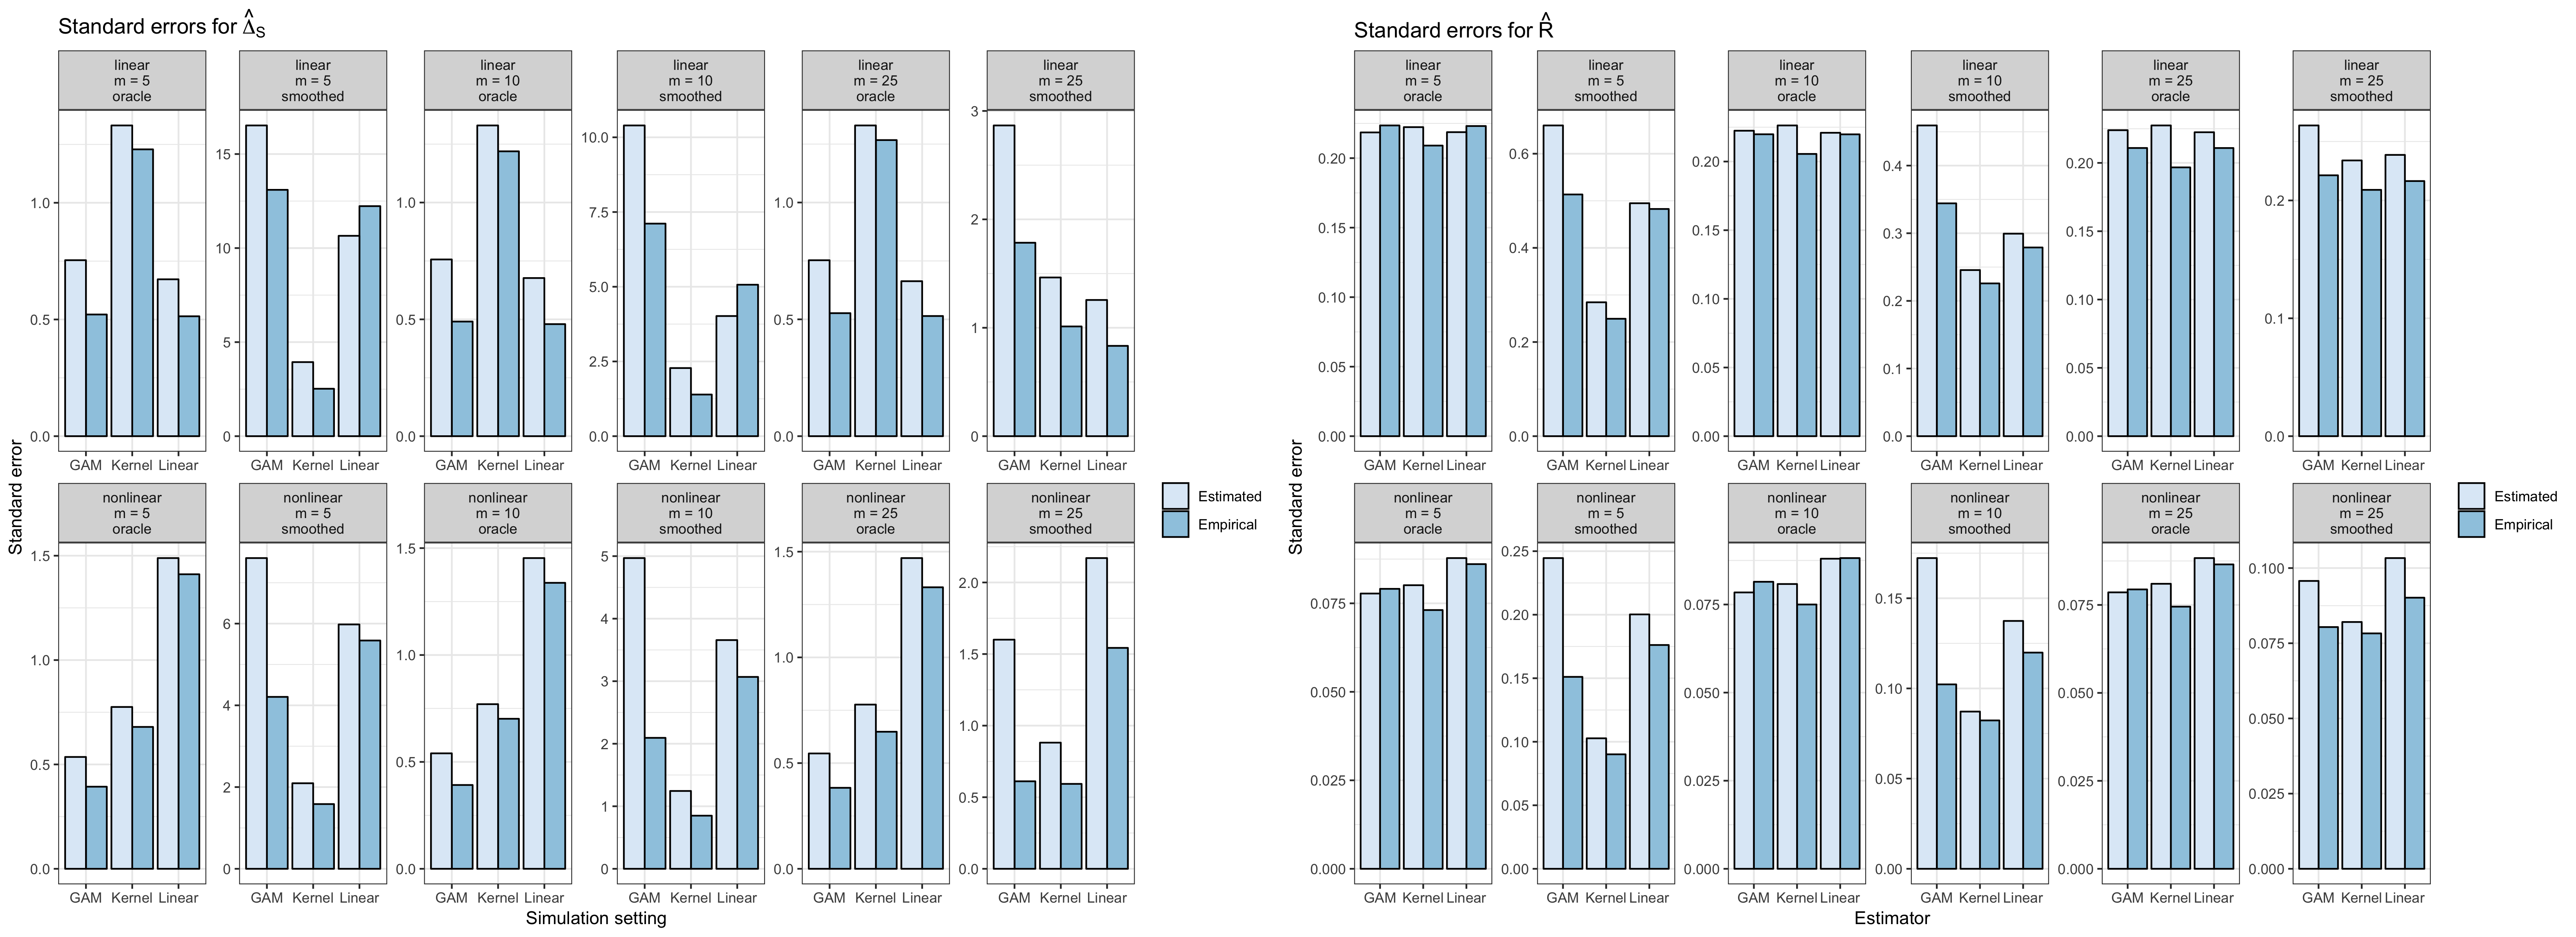
\includegraphics[width =\textwidth]{results/standard-error-figure.png}
\end{tabular}\vspace{0.2in}
\caption{Standard errors for $\Deltahat_S$ and $\Rhat$ using each of the proposed estimators and 250 bootstrap samples. Sample size was set to $n = 50$, and $\Delta_S = 25$.}\label{fig:se}
\end{figure}

We further show in Figure \ref{fig:ci} that confidence interval coverage exceeds the nominal level for 

\begin{figure}
\centering
\begin{tabular}{c}
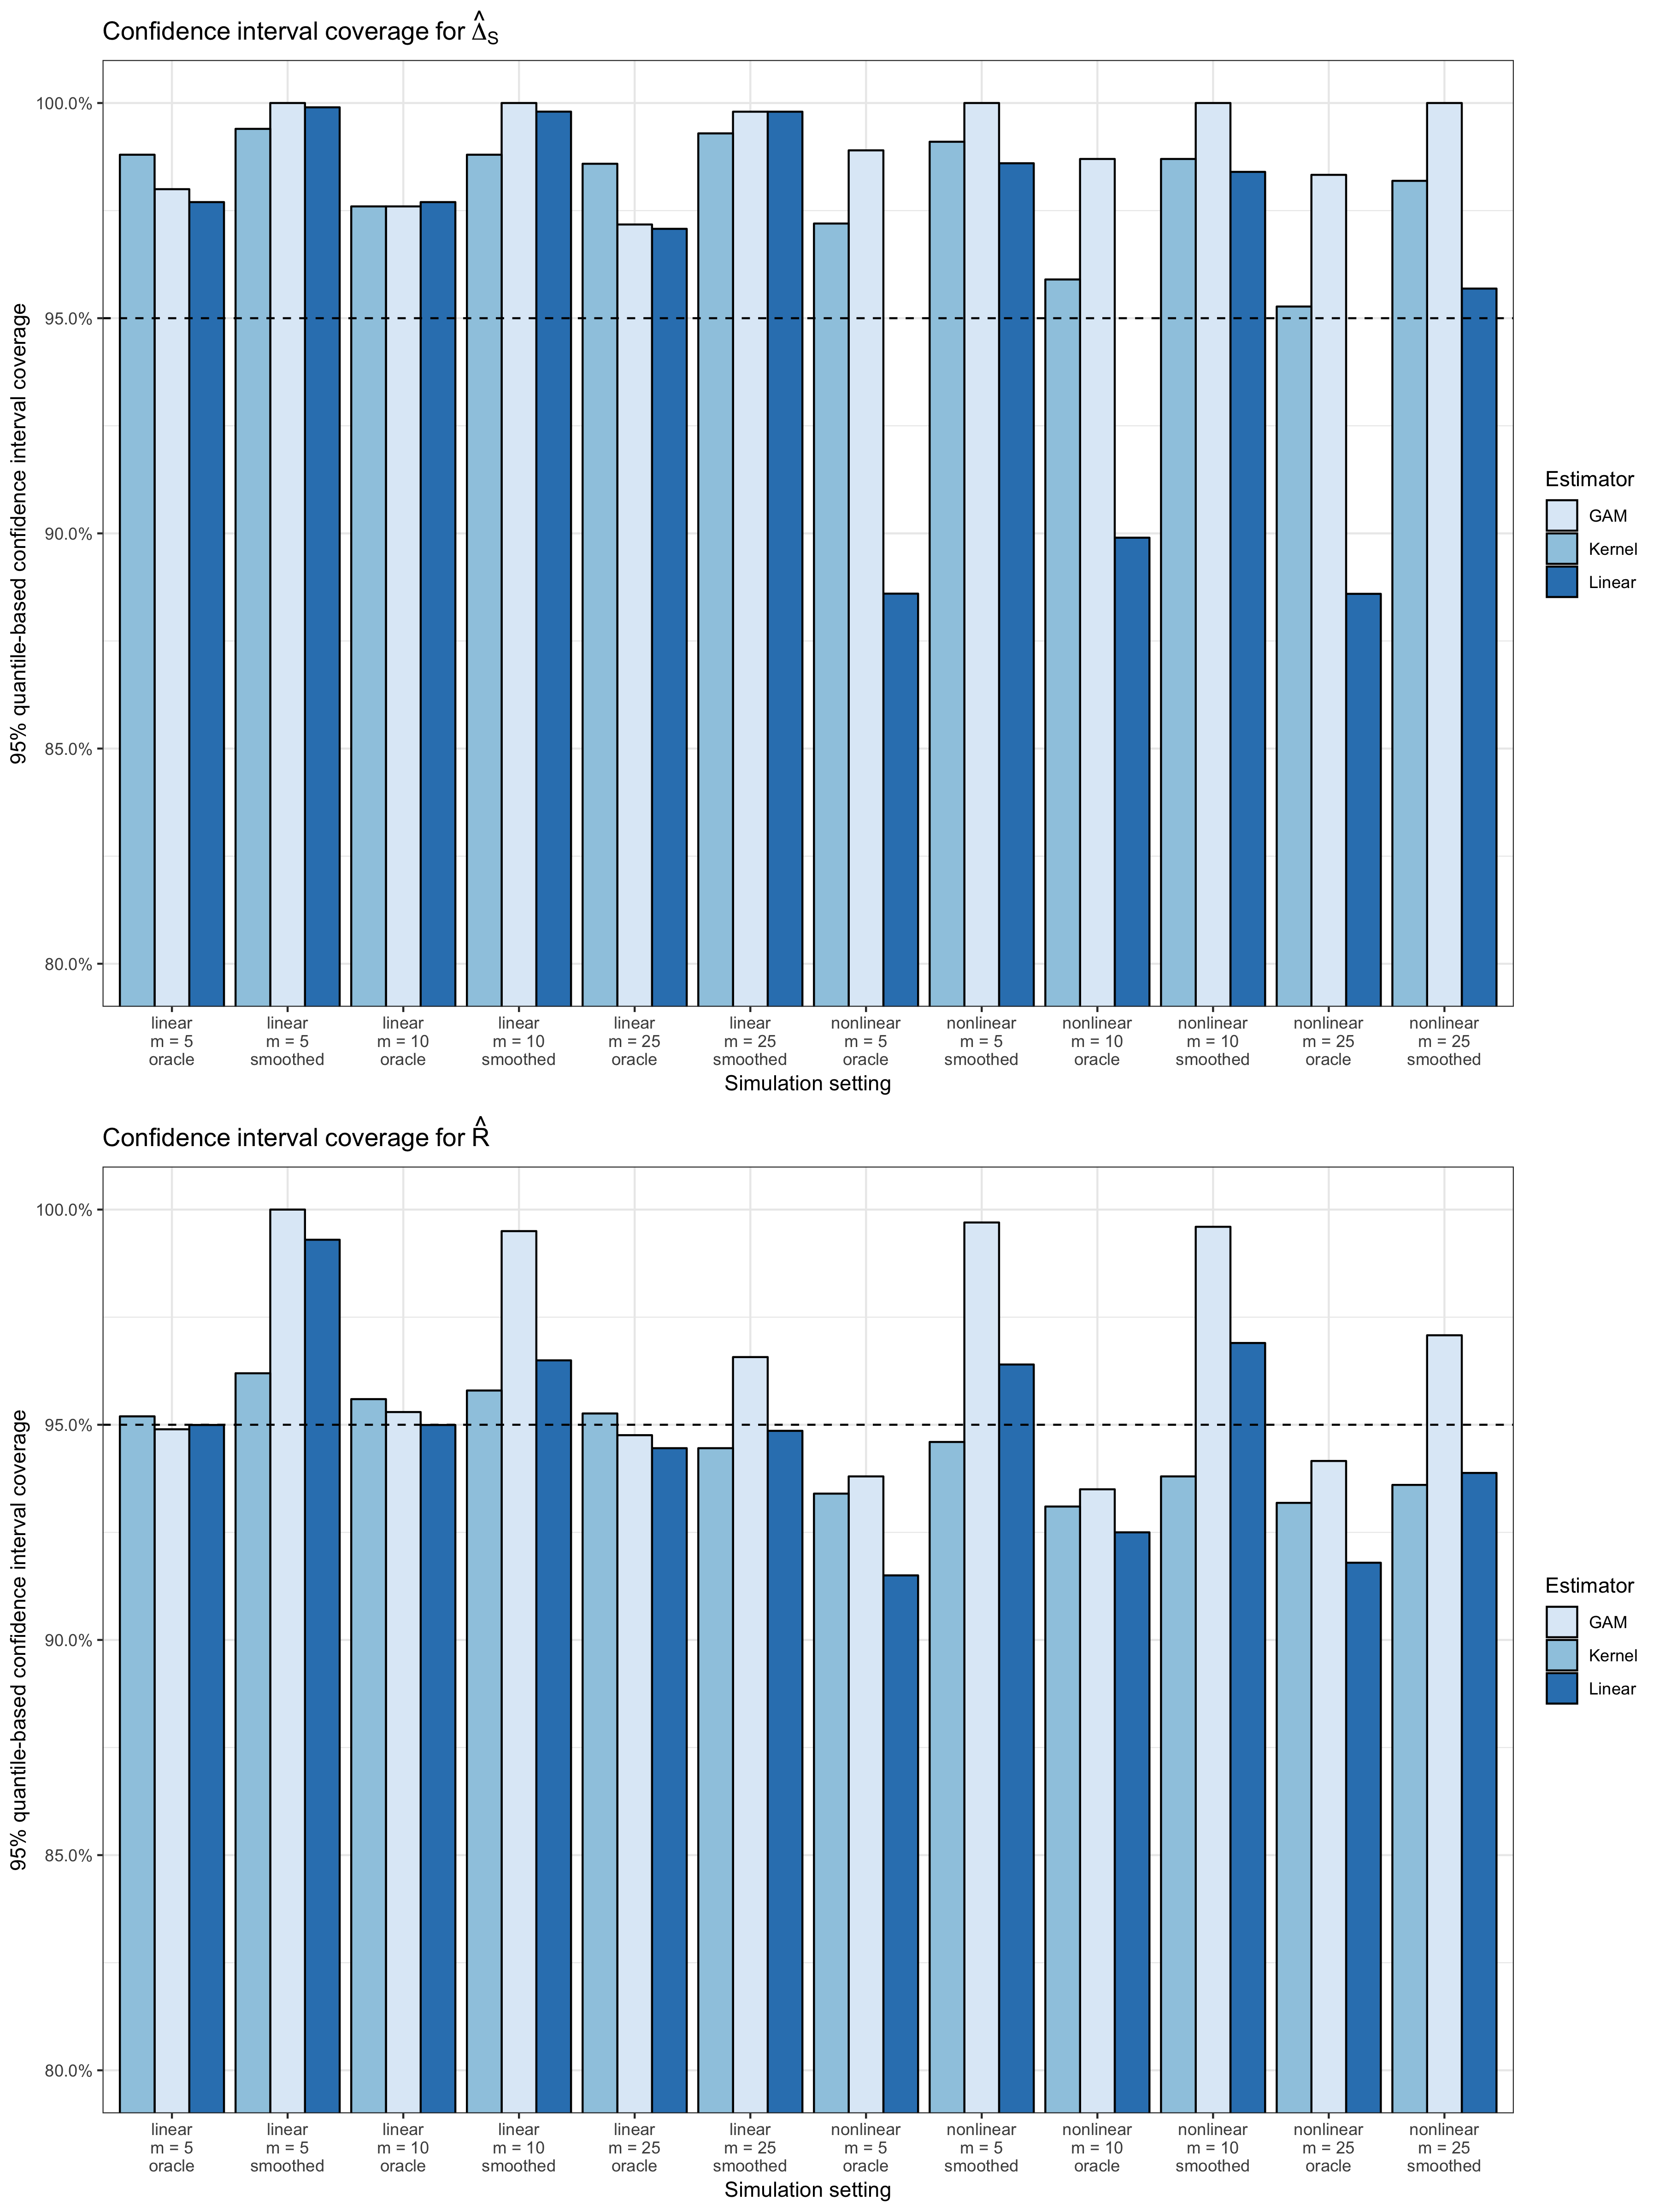
\includegraphics[width =\textwidth]{results/quantile-ci-figure.png}
\end{tabular}\vspace{0.2in}
\caption{95\% quantile-based confidence interval coverage for $\Delta_S$ and $R$ based on the proposed estimators using 250 bootstrap samples. Sample size was set to $n = 50$, and $\Delta_S = 25$.}\label{fig:ci}
\end{figure}


\section{Analysis of longitudinal CD4 count
surrogacy}\label{analysis-of-longitudinal-cd4-count-surrogacy}

We illustrate the proposed procedures using a dataset from the AIDS Clinical Trial Group (ACTG) Protocol 175 \citep{Hammer96}. This study enrolled 2,467 patients randomized to 4 different treatments: zidovudine only, zidovudine + didanosine, zidovudine + zalcitabine, and didanosine only. We seek to quantify the extent to which CD4 counts measured in the first year after randomization capture the treatment effect on a longer term outcome.

The primary outcome was the difference between CD4 count at 2 years after randomization and the mean of two CD4 count measurements at baseline. Patients who did not have a CD4 count measured within 90 days of 2 years of post-randomization, possibly because they were censored, died, or experienced an AIDS-defining event before that time were not analyzed. We let the surrogate marker be CD4 count measured between two weeks prior to randomization and one year post-randomization. We furthermore focused on comparing the zidovudine-only treatment group to the zidovudine + didanosine. This left a total of 460 individuals in the zidovudine + didanosine group, each having on average 6.4 longitudinal surrogate CD4 observations within the first year after randomizations, and 427 individuals in the zidovudine-only group, each having 6.6 CD4 surrogate observations on average. 

We compared our estimators to two naive approaches which take the surrogate to be other summaries of the CD4 counts in the year after randomization: one uses the mean of the CD4 counts, and the other uses the change from the first measurement of CD4 to the last measurement prior to a year after randomization. For the longitudinal surrogate estimators, $\Deltahat_S\lin, \Deltahat_S\gam$, and $\Deltahat_S\k$, CD4 surrogate data were pre-smoothed using FPCA. Cross validation was used to select the bandwidth for the mean function, while the default method of 10\% of the support was used for the covariance function. AIC was used to select the number of included principal components. Cross validation was used to select the bandwidths for the kernel estimators. 

The mean change in CD4 count at 2 years after randomization was -15.0 for patients randomized to zidovudine + didanosine, while the mean change in the zidovudine-only group was -92.0, making the overall treatment effect estimate 77.0. Using a linear working model, we estimated the residual treatment effect to be $\Deltahat_S\lin = 21.0$ and the proportion of the treatment effect explained by first-year CD4 measurements to be $\Rhat\lin = 0.73$, suggesting these first-year measurements are quite good surrogates for the later outcome. The more flexible additive model suggested that the residual treatment effect was even lower $\Deltahat_s\fgam = 8.8$ and the proportion explained even higher $\Rhat\fgam = 0.89$. The fully nonparametric estimator on the other hand suggested that the degree of surrogacy was much lower, with $\Deltahat_S\k = 42.0$ and $\Rhat\k = 0.46$. The naive methods also gave much lower estimates of longitudinal CD4 surrogacy. The estimated proportion of the treatment effect explained by the mean CD4 count was 0.18, and the proportion explained by the change was 0.55. 



\section{Discussion}\label{discussion}
Assessing the surrogacy of a longitudinal marker trajectory is important for identifying promising surrogate markers for future studies; limited methods exist to define and estimate quantities that achieve this goal. We proposed a definition of the proportion of treatment effect explained by a surrogate marker trajectory and three novel flexible methods to estimate this defined quantity. Our methods demonstrate good performance and finite sample properties. An R package available on CRAN, \texttt{Rsurrogate}, implements the three methods proposed here. \textcolor{red}{Layla will need to add these functions before submission.}

Our approach does have some limitations. We initially require the assumption that $\bX_i$ is observed on a common dense grid though this often needs to be estimated in practice. 

Extension of our approach to a time-to-event outcome setting with potential censoring is certainly warranted. In the AIDS study, for example, while CD4 count is itself often used as a primary outcome, it would be of interest to develop these procedures such that the primary outcome of time to death or an aids defining event could be examined. This, however, is not a trivial extension. Besides potential censoring which will likely need to be accommodated, it is likely that individuals may experience the outcome of interest e.g. death early in the study, as the surrogate marker trajectory is being measured. In this case, careful consideration is needed to decide whether and how the surrogate trajectory before death and/or the observed death time will be handled in this framework.

\section*{Acknowledgements}
Support for this research was provided by National Institutes of Health grant R01HL088589. We thank the AIDS Clinical Trial group for providing the example data. 

\clearpage
\bibliographystyle{biom}
\bibliography{bibliography.bib}

\section{Appendix}
\textcolor{red}{(Add conditions and assumptions needed.)}
Let $\pi_j = \frac{n_j}{n} > 0, j = 0,1$. $\bX\sone$ and $\bX\szero$ are $d$-dimensional realizations of random functions on a compact interval $\Isc$. Let $F\sone, F\szero$ be the distribution functions for the surrogates in the treated and control groups respectively, and let $f\sone, f\szero$ be the respective densities. We assume the support of $\bX\sone$ contain the support of $\bX\szero$, $\text{supp}(\bX\sone) = \{\bx : f\sone(\bx) > 0\} \supset \text{supp}(\bX\szero) = \{\bx : f\szero(\bx) > 0\}$. Further {\color{red} let $\mu_1(\bx)r(\bx)$ have continuous second derivatives over $\text{supp}(\bX\sone)$} where $r(\bx) = f\szero(\bx)/f\zone(\bx)$. Finally, we take the kernel function $K(x)$ to be a smooth function with finite support, symmetric at zero and $\int K(x)dx) = 1$. Let $K_h(x) = K(s/h)/h$ where $h$ is a smoothing bandwidth assumed to be $O_p(n^{-\delta}), \delta \in (1/4, 1/2)$. 

\subsection{Asymptotics of linear estimator}
Proof of Theorem 1. We require the following
\begin{enumerate}
    \item Both $\bX\sone$ and $\bX\szero$ are bounded, and the random variables $\bbeta_0\trans\bX\sone$ and $\bbeta_0\trans\bX\szero$ have continuous density functions $f\sone_{\bbeta_0}$ and $f\szero_{\bbeta_0}$ with finite support and $\text{supp}(\bX\szero) \subset \text{supp}(\bX\sone) \subset [a,b]$. 
    \item Let $\mu\sone_{\bbeta}(u) = E(Y\sone | \bbeta\trans\bx = u$ and $r_{\bbeta}(u) = f\szero_{\bbeta}(u) / f\sone_{\bbeta}(u)$. The function $\mu\sone{\bbeta_0}(u)r_{\bbeta_0}(u)$ has a continuous second derivative over $[a,b]$.
    \item For sufficiently small $\delta > 0$,
    \begin{align*}
        |r_{\bbeta_2}(u) - r_{\bbeta_1}(u)| + |\mu_{\bbeta_2}\sone(u)r_{\bbeta_2}(u) - \mu_{\bbeta_1}\sone(u)r_{\bbeta_1}(u)| \leq C_0|\bbeta_2 - \bbeta_1|
    \end{align*}
    for $|\bbeta_i - \bbeta_0| < \delta, i = 1,2.$ ({\color{red} does this need to be a norm?}).
    \item $n\inv R_\rho \rightarrow 0, (nR_\rho\inv) \rightarrow 0$ ({\color{red} check rate of $R_\rho$})
\end{enumerate}.

We verify that \begin{align*}
    n_1^{-\frac{1}{2}}(\bbetahat - \bbeta_0) = n_1^{-\frac{1}{2}}\sumin \tau_i + o_p(1)
\end{align*}
where $\tau_i = E\subxo(\bXtilde\bXtilde\trans + R_\rho)\inv\bXtilde_i Y_iI\{A_i = 1\}$, $E(\tau_i) = 0,$ and $E(\tau_i^2) < \infty$, so that $|\bbetahat - \bbeta_0| = O_p(\nnhalf).$

The proof then follows from the result in Appendix C of \cite{parast2016robust}, where it is shown that 
\begin{align*}
    \nhalf\left(
    \begin{matrix}
    \Deltahat_S\lin - \Delta_S\lin\\
    \Deltahat - \Delta
    \end{matrix}
    \right) \rightarrow N(0, \Sigma)
\end{align*}
where $\Sigma = \Sigma_1 + \Sigma_0$ and $\Sigma_1 = \pi_1\inv E_{Y\sone,\bX\sone}\left(
    \begin{matrix}
    \left\{Y - m_1(\bX\trans\bbeta_0)\right\}r(\bX\trans\bbeta_0) + \ba_0\trans\tau\\
    Y - E_{Y\sone}(Y)
    \end{matrix}
    \right),
    
    \Sigma_0 = \pi_0\inv E_{Y\szero,\bX\szero}\left(
    \begin{matrix}
    Y - E_{Y\szero}(Y) - m_1(\bX\trans\bbeta_0) + \int m_1(x)F_0\\
    Y - E_{Y\sone}[Y]
    \end{matrix}
    \right)
    $

\subsection{Asymptotics of kernel-based estimator}
Proof of Theorem 3. Recall that $\Deltahat_S = \Ehat_{\bX\szero}\left \{ \Ehat(Y\sone| \bX\sone =\bx)\right \} - \Ehat(Y\szero) = \Ehat_{\bX\szero}\left \{ \mhat_1(\bX)\right \} - \Ehat(Y\szero)$. To establish the consistency of $\Deltahat_S$ it is sufficient to show that 
\begin{align*}
    \Ehat_{\bX\szero}\left \{ \mhat_1(\bX)\right \} - E_{\bX\szero}\left \{ m_1(\bX)\right \} = o_p(1)
\end{align*}
Note that by the strong law of large numbers $\left|\Ehat_{\bX\szero}\left \{ m_1(\bX)\right \} - E_{\bX\szero}\left \{ m_1(\bX)\right \}\right| = o_p(1)$, and recall that $\var\{\mhat(\bX) - m(\bX)\} = O_p\left[\{n\Fhat(h)\}\inv\right] = o_p(1)$. So,
\begin{align*}
    &\left|\Ehat_{\bX\szero}\left \{ \mhat_1(\bX)\right \} - E_{\bX\szero}\left \{ m_1(\bX)\right \}\right| \leq\\ &\qquad\left|E_{\bX\szero}\left \{ \mhat_1(\bX) - m_1(\bX)\right\}\right| + \left|\Ehat_{\bX\szero}\left \{ m_1(\bX)\right \} - E_{\bX\szero}\left \{ m_1(\bX)\right \}\right| +\\ &\qquad\left|\Ehat_{\bX\szero}\left \{ \mhat_1(\bX) - m_1(\bX)\right\} - E_{\bX\szero}\left \{ \mhat_1(\bX) - m_1(\bX)\right\}\right|\\
    &= o_p(1)
\end{align*}
because of the uniform consistency of $\mhat(\bX)$ and the strong law of large numbers. {\color{red} this needs to be formalized in terms of moment conditions.}

To establish asymptotic normality, we first write the asymptotic distribution of \begin{align*}
    &\nhalf\left[\Ehat_{\bX\szero}\left \{ \mhat_1(\bX)\right \} - E_{\bX\szero}\left \{ m_1(\bX)\right \}\right]\\
     &=\quad \nhalf\left[E_{\bX\szero}\left \{ \mhat_1(\bX) - m_1(\bX)\right\}\right] + \nhalf\left[\Ehat_{\bX\szero}\left \{ m_1(\bX)\right \} - E_{\bX\szero}\left \{ m_1(\bX)\right \}\right] +\\ &\quad\nhalf\left[\Ehat_{\bX\szero}\left \{ \mhat_1(\bX) - m_1(\bX)\right\} - E_{\bX\szero}\left \{ \mhat_1(\bX) - m_1(\bX)\right\}\right]\\
     &= \quad \nhalf\left[E_{\bX\szero}\left \{ \mhat_1(\bX) - m_1(\bX)\right\}\right] + \nhalf\left[\Ehat_{\bX\szero}\left \{ m_1(\bX)\right \} - E_{\bX\szero}\left \{ m_1(\bX)\right \}\right] + o_p(\nnhalf)
\end{align*}
because $Z_i = \mhat_1(\bX) - m_1(\bX) - E_{\bX\szero}\left \{ \mhat_1(\bX) - m_1(\bX)\right\}$ has $E[Z_i] = 0, \var(Z_i) = o_p(1).$

Taking the first term $\nhalf\left[E_{\bX\szero}\left \{ \mhat_1(\bX) - m_1(\bX)\right\}\right]$ first. Let $f_1(\bx) = E_{\bX\sone}[K\{d(\bx, \bX_i)/h\}]$ consider that
\begin{align*}
    &\nhalf\left[E_{\bX\szero}\left \{ \mhat_1(\bX) - m_1(\bX)\right\}\right] = \nhalf \left[E_{\bX\szero}\left \{ \frac{\sumin K\{d(\bX, \bX_i)/h\}Y_iI\{A_i = 1\}}{\sumin K\{d(\bX, \bX_i)/h\}I\{A_i = 1\}}  - m_1(\bX)\right\}\right]\\
    &= \nhalf E_{\bX\szero}\left \{m_1(\bX)n_1\inv\sum_{i : A_i = 1}\left[\frac{K\{d(\bX, \bX_i)/h\}}{f_1(\bX)} - 1\right] + n_1\inv\sum_{i : A_i = 1}\frac{K\{d(\bX, \bX_i)/h\}Y_i}{f_1(\bX)} - m_1(\bX)
    \right\} + O_p(\text{\color{red} fill in rate})
\end{align*}
because of the uniform consistency of $\mhat_1(\cdot)$ {\color{red} give this result somewhere}. 
\begin{align*}
    &\nhalf\left[E_{\bX\szero}\left \{ \mhat_1(\bX) - m_1(\bX)\right\}\right] = \\
    &(n_1\pi_1)\mhalf\sum_{i : A_i = 1}E\subxz\left(\frac{m_1(\bX)}{f_1(\bX)}\left\{K\{d(\bX, \bX_i)/h\} - f_1(\bX)\right\} + \left[\frac{Y_iK\{d(\bX, \bX_i)/h\}}{f_1(\bX)} \right] \right) + o_p(1)
\end{align*}
Now,
\begin{align*}
    &(n_1\pi_1)\mhalf\sum_{i : A_i = 1}E\subxz\left(\frac{m_1(\bX)}{f_1(\bX)}\left\{K\{d(\bX, \bX_i)/h\} - f_1(\bX)\right\}\right)\\
    &= 
\end{align*}

%\cite{Vieu2016} show that under suitable regularity conditions
%\begin{align*}
%    \sqrt{\frac{n\Fhat(h)M_1^2}{\sigma^2M_1}}\{\mhat(\bx) - m(\bx)\} \rightarrow N(0,1)
%\end{align*}
% We need the distribution of $\alpha_n(\Deltahat_s - \Delta_S) = \alpha_n\left(n_0\inv\sum_{i : A_i = 0}\mhat(\bX_i) - \Ybar_0\right)$
\label{lastpage}

\end{document}
